%%%%%%%%%%%%%%%%
%
% File Manual_Cyclic_en.tex
% English manual for the entire ``Cyclic'' project
% Created: March 26, 2021, Alex
% Edited: March 26, 2021, Alex
% Edited: March 30, 2021, Haraguchi
%
%%%%%%%%%%%%%%%%%%%%%%%

\documentclass[11pt,titlepage,dvipdfmx,twoside]{book}
\linespread{1.1}

\usepackage{amsfonts}
\usepackage{amssymb}
\usepackage{amsmath}
\usepackage{amsthm}
\newtheorem{theorem}{Theorem}
\newtheorem{lemma}[theorem]{Lemma}
\usepackage{enumitem}
\usepackage{geometry}
\geometry{left=2.5cm,right=2.5cm,top=2.5cm,bottom=2.5cm}

\usepackage{algorithm}  
\usepackage{algorithmic}  
\renewcommand{\algorithmicrequire}{\textbf{Input:}} 
\renewcommand{\algorithmicensure}{\textbf{Output:}}
\renewcommand{\algorithmicforall}{\textbf{for each}}

\usepackage{mathtools}
\usepackage{comment}
\usepackage[dvipdfmx]{graphicx}
\usepackage{float}
\usepackage{framed}
\usepackage{graphicx}
\usepackage{subcaption}
\usepackage{color}
\usepackage{url}
\newenvironment{myframe}{\begin{trivlist}\item[]
    \hrule
    \hbox to \linewidth\bgroup
    \advance\linewidth by -30pt
    \hsize=\linewidth
    \vrule\hfill
    \vbox\bgroup
    \vskip15pt
    \def\thempfootnote{\arabic{mpfootnote}}
    \begin{minipage}{\linewidth}}{%
    \end{minipage}\vskip15pt
    \egroup\hfill\vrule
    \egroup\hrule
\end{trivlist}}

\usepackage{dirtree}

\newcommand{\project}{{\tt mol-infer/Cyclic}}
\newcommand{\chapref}[1]{Chapter~\ref{chap:#1}}
\newcommand{\secref}[1]{Section~\ref{sec:#1}}
\newcommand{\tabref}[1]{Table~\ref{tab:#1}}
\newcommand{\figref}[1]{Figure~\ref{fig:#1}}
\long\def\invis#1{}

%%%%%%%%%%%%%%%%%%%%%%%%%%%%%%%%%%%%%%%%%%%%%%%%%%%%%%%%%%%%


\title{\huge{
Chemical Graph Project: \\
Inferring Cyclic Chemical Graphs}}

\author{\project}

\begin{document}

\pagenumbering{roman}

% \西暦
\date{\today}

\maketitle


\hfill

\chapter*{Introduction}

\section*{Abstract}
Our research goal is to develop a system
that generates chemical graphs such that
the corresponding compounds must attain
a desired value for a prescribed chemical property.
This system consists of four modules as follows.
\begin{description}
\item[Module 1:]
Converting a given data on chemical graphs
  (represented by an SDF file) into a set of feature vectors.
  
\item[Module 2:] 
Training an Artificial Neural Network by using the set of feature vectors as the training set. 

\item[Module 3:] 
Inferring a chemical graph that must attain a desired 
property value by using mixed integer linear programming. 

\item[Module 4:] 
Listing chemical isomers of the chemical graph obtained in Module 3. 
\end{description}

This booklet explains how to obtain inferred chemical graphs
by using the programs of the modules.

\section*{Structure of Files and Folders}
\dirtree{%
.1 .
.2 LICENSE.
.2 Makefile.
.2 README.md.
.2 bin.
.3 cyclic\_graphs\_MILP\_ec\_id.py.
.3 .DS\_Store.
.3 infer\_cyclic\_graphs\_ec\_id.py.
.3 ann\_inverter.py.
.3 predict\_values.py.
.3 mol-infer\_ANN.py.
.3 eliminate.py.
.3 read\_instance\_BH\_cyclic.py.
.3 osx.
.4 generate\_isomers.
.4 CHECKER.
.4 FV\_ec.
.4 generate\_partition.
.4 FV\_proj.
.3 linux.
.4 generate\_isomers.
.4 CHECKER.
.4 FV\_ec.
.4 generate\_partition.
.4 FV\_proj.
.2 doc.
.3 cyclic\_flow.pdf.
.3 Manual\_Cyclic\_en.pdf.
.3 Manual\_Cyclic\_jp.pdf.
.2 instances.
.3 chemical\_specification.
.4 instance\_b4.txt.
.4 instance\_a.txt.
.4 instance\_c.txt.
.4 instance\_b2.txt.
.4 instance\_b3.txt.
.4 instance\_b1.txt.
.4 instance\_d.txt.
.3 BP.
.4 BP\_desc.csv.
.4 BP\_GEN.sdf.
.4 BP\_values.txt.
.4 BP\_MILP.LOG.
.4 BP\_MILP\_partition.txt.
.4 BP\_ANN.LOG.
.4 BP.sdf.
.4 BP\_biases.txt.
.4 BP\_weights.txt.
.4 BP\_MILP.sdf.
.4 BP\_GEN.LOG.
.3 KOW.
.4 KOW\_GEN.sdf.
.4 KOW\_MILP.LOG.
.4 KOW\_values.txt.
.4 KOW\_MILP\_partition.txt.
.4 KOW\_desc.csv.
.4 KOW\_weights.txt.
.4 KOW\_GEN.LOG.
.4 KOW\_MILP.sdf.
.4 KOW\_biases.txt.
.4 KOW.sdf.
.4 KOW\_ANN.LOG.
.3 MP.
.4 MP\_values.txt.
.4 MP\_GEN.LOG.
.4 MP.sdf.
.4 MP\_ANN.LOG.
.4 MP\_MILP.sdf.
.4 MP\_weights.txt.
.4 MP\_desc.csv.
.4 MP\_biases.txt.
.4 MP\_GEN.sdf.
.4 MP\_MILP.LOG.
.4 MP\_MILP\_partition.txt.
.2 src.
.3 Module\_1.
.4 fv\_proj.cpp.
.4 cycle\_checker.cpp.
.4 fv\_ec.cpp.
.4 eliminate.py.
.3 Module\_2.
.4 predict\_values.py.
.4 mol-infer\_ANN.py.
.3 Module\_3.
.4 cyclic\_graphs\_MILP\_ec\_id.py.
.4 infer\_cyclic\_graphs\_ec\_id.py.
.4 ann\_inverter.py.
.4 read\_instance\_BH\_cyclic.py.
.3 Module\_4.
.4 include.
.5 cross\_timer.h.
.5 fringe\_tree.hpp.
.5 tools.hpp.
.5 chemical\_graph.hpp.
.5 data\_structures.hpp.
.4 main.
.5 generate\_partition.cpp.
.5 generate\_isomers.cpp.
}
% \cleardoublepage

\pagestyle{plain}
\tableofcontents
\clearpage

\pagenumbering{arabic}


\chapter{Module 1: Calculating a Feature Vector from an SDF File}


\section{Introduction}
This chapter serves as a manual and
explains the procedures to run Module~1 of the \project\ project.
The input and output of Module~1 are as follows.

\begin{oframed}
\begin{description}
\item[Input:] 
A set $D=\{G_1, G_2, \dots, G_p\}$ of cyclic chemical graphs. 
%
\item[Output:] 
A set ${\mathcal F}(D)\triangleq\{f(G_1), f(G_2), \dots, f(G_p)\}$
of feature vectors, such that $f(\cdot)$ is a feature vector of
chemical graphs as details in the accompanying article~\cite{AN20}.
%
\end{description}
\end{oframed}
%
The output is written to a csv (comma-separated value) file.
This csv file is used in Module~2 of the project.


The remainder of this chapter is organized as follows. 
\begin{itemize}
\item \chapref{preparation}: 
Summary of essential terminology. %, as well, as the file organization in this package.

\item \chapref{quick}: 
A short computational example.

\item \chapref{io}: 
Detailed explanations of the program's input and output.
\end{itemize}

%%%%%%%%%%%%%%%%%%%%%%%%%%%%%%%%%%%%%%%%%%%%%%%%%%%%%%%%%%%%
%\clearpage
\section{Preliminaries}
\label{chap:preparation}

%\subsection{Terminology}
\paragraph{Chemical Graph.}
A {\bf graph} is an abstract combinatorial construction
comprising a set of {\bf nodes} and a set of {\bf edges},
where an edge is an unordered pair of nodes.
A {\bf cycle} in a graph is a sequence of
nodes such that except for the first and the last node,
each node is unique, and there is an edge in the graph 
for each pair of consecutive 
nodes in the sequence.

A graph where each node is assigned a chemical element
(such as carbon, nitrogen, oxygen, etc.) and each
edge is assigned a multiplicity between 1 and 4,
is called a {\bf chemical graph}.


\paragraph{Descriptor.}
A {\bf descriptor} is a numerical value that 
indicates a certain characteristic of a chemical graph.
In this project, among others, descriptors include
the number of non-hydrogen atoms, the number of atoms in the core of the 
chemical graph, the core height, etc.
For a complete list of descriptors, please refer to the 
accompanying article~\cite{AN20}.


\paragraph{Feature vector.}
A vector that comprises the numerical values for
the descriptors of a chemical graph.


\invis{
\subsection{File Structure}
The following set of files accompany this note.
\begin{itemize}
\item {\tt Makefile}: 
A makefile for compiling the programs. 
%
\item {\tt cycle\_checker.cpp}: 
Source code written in C++ that for a given chemical compound checks if 
the chemical graph contains a cycle or not
%.  
\item {\tt eliminate.py}: 
A Python script that screens chemical compounds that are not
considered under this project, such us inorganic
compounds with less than four carbon atoms, 
that contain charged atoms, etc.
%
\item {\tt fv\_ec.cpp}: 
Source code written in C++ 
of the mail program of Module~1,
calculating a feature vector.
%
\item {\tt fv\_proj.cpp}: 
Source code (C++) of a program
that given a feature vector function $f$
calculated over a set $D$ of chemical graphs,
and a set $D'$ of chemical graphs that does not necessarily have the same
descriptors as $D$ does, 
calculates the set ${\mathcal F}(D')$ of feature vectors
projected onto the domain of~$f$.
This is an auxiliary program, 
and usually not essential to the flow of the entire project.
%
\item Folder {\tt data} 
Contains sample input and output files
used to test and demonstrate the execution of the
programs in Module~1.
The files in this folder as as follows.
%
\begin{itemize}
  \item {\tt sample1.sdf}: 
  An SDF file that contains a single chemical compound.
  (Please check \chapref{io} for more details on SDF files.)
  %
  \item {\tt sample1\_eli.sdf}: 
  An SDF file obtained as the output of the Python script 
  {\tt eliminate.py} when invoked on the file {\tt sample1.sdf}.
  The contents of the files {\tt sample1.sdf} and {\tt sample1\_eli.sdf}
  should be identical.
  %
  \item {\tt sample1.csv}: 
  Contains a single feature vector
  constructed from the file
  {\tt sample1\_eli.sdf}.
  %
  \item {\tt sample2.sdf}: 
  An SDF file that contains data on 175 chemical graphs.
%
  \item {\tt sample2\_eli.sdf}: 
    An SDF file obtained as the output of the Python script 
  {\tt eliminate.py} when invoked on the file {\tt sample2.sdf}.
  The contents of the files {\tt sample2.sdf} and {\tt sample2\_eli.sdf}
  should be identical.
  %
  \item {\tt sample2.csv}: 
  Contains the set of feature vectors
  constructed from the file
  {\tt sample2\_eli.sdf}.
  %
  \item {\tt sample1\_on\_2.csv}: 
  Contains a single feature vector whose values are calculated
  from the file
  {\tt sample1\_eli.sdf},
  however, the dimensions of the vector are projected 
  on the domain of the feature vector obtained from
  the file {\tt sample2\_eli.sdf}. 
  \end{itemize}
\end{itemize}
}

%%%%%%%%%%%%%%%%%%%%%%%%%%%%%%%%%%%%%%%%%%%%%%%%%%%%%%%%%%%%
%\clearpage
\section{Execution Example}
\label{chap:quick}

\subsection{Validation of the Data}
%
Data on chemical compounds (equivalently, chemical graphs) is stored in a standard SDF file
(more information on the structure of SDF files is given in \chapref{io}).
Each chemical graph~$G$ 
must satisfy the following conditions
%
\begin{description}
\item[(i)] 
 $G$ must contain a cycle;
%
\item[(ii)] 
 $G$ must contain at least four carbon atoms,
 none of the atoms is allowed to be charged,
 and each atom must have atomic mass as listed
 in~\chapref{caution}; and
 %
\item[(iii)] Must not include an aromatic edge.
\end{description}
%

The Python script {\tt eliminate.py}
%included in Module~1
can be used to remove the graphs that do not satisfy 
condition~(ii). % and~(iii).
For condition (iii),
the user must confirm whether it is satisfied or not
on his/her own. 

\paragraph{Confirming that a chemical graph contains a cycle.}
%
Please use the program compiled from the source file  
{\tt cycle\_checker.cpp}
included in Module~1 to confirm whether each chemical graph in a given
SDF file contains a cycle.

A compiled executable is included in the folder {\tt bin},
for each of the following operating systems:
%
\begin{itemize}
 \item [--] linux
 \item [--] osx
 \item [--] windows (cygwin).
\end{itemize}

In addition, the user can compile the accompanying source files.
To compile the program, the included {\tt Makefile}
can be used by issuing the following command in the command prompt.
\begin{oframed}
{\small
\verb|$ make CHECKER|
}
\end{oframed}
%
In case the {\tt make} command is not available on the system,
then the program can be compiled in the following way.
\begin{oframed}
{\small
\verb|$ g++ -std=c++11 -O3 -o CHECKER cycle_checker.cpp|
}
\end{oframed}

In order to check if a given
SDF file {\tt input.sdf} contains a chemical graph that does not include
a cycle by issuing the following command on the terminal.
\begin{oframed}
{\small
\verb|$ ./CHECKER input.sdf|
}
\end{oframed}


\begin{itemize}
\item If all chemical graphs have cycles
  (i.e., all satisfy (i)),
  then the program CHECKER does not output any message.
  In this case, one can go to the next step. 
\item Otherwise, (i.e., there is a chemical graph that does not satisfy (i)),
  the CID of such a chemical graph is output.
  Before going to the next step,
  such a graph must be removed from the SDF file manually.  
\end{itemize}

\paragraph{Elimination of chemical graphs that are out-of-scope.}
To check whether each chemical graph in a given SDF file
satisfies condition (ii) or not,
please use the Python script named 
{\tt eliminate.py}.
The script generates a new SDF file
that consists of all chemical graphs in the input SDF file
that satisfy (ii). 

To use {\tt eliminate.py}, execute the following command. 

\begin{oframed}
{\small
\verb|$ python eliminate.py input.sdf|
}
\end{oframed}

If the {\tt input.sdf} contains a chemical graph
that does not satisfy (ii), the CID is printed.

After the execution of {\tt eliminate.py},
a new SDF file {\tt input\_eli.sdf} is created.
The file consists of all chemical graphs in {\tt input.sdf}
that satisfy condition (ii).
%
This means that, if all chemical graphs in {\tt input.sdf}
satisfy (ii), then
{\tt input.sdf} and {\tt input\_eli.sdf} are equivalent. 


\subsection{Calculating a Feature Vector}
Please use the program compiled from the source file
{\tt fv\_ec.cpp} %included in Module~1
to calculate feature vectors for an SDF file
such that every chemical 
satisfies conditions (i), (ii), and (iii).

Again, a compiled executable is included in the folder {\tt bin},
for each of the following operating systems:
%
\begin{itemize}
 \item [--] linux
 \item [--] osx
 \item [--] windows (cygwin).
\end{itemize}

To compile the program, the included {\tt Makefile}
can be used by issuing the following command in the
command prompt. 
\begin{oframed}
{\small
\verb|$ make FV_ec|
}
\end{oframed}
%
In case the {\tt make} command is not
available on the system,
then the program can be compiled in the following way. 
\begin{oframed}
{\small
\verb|$ g++ -std=c++11 -O3 -o FV_ec fv_ec.cpp|
}
\end{oframed}


In order to calculate feature vectors from {\tt input\_eli.sdf} and to output the result in {\tt output.csv},
issue the following command on the terminal. 
\begin{oframed}
{\small
\verb|$ ./FV_ec input_eli.sdf output.csv|
}
\end{oframed}
The program {\tt FV\_ec} prints on the terminal instructions on how to provide the arguments
and halts if the arguments are not provided appropriately.

\subsection{Calculating a Feature Vector from Other SDF (Not Mandatory)}

The mapping $f$ that transforms a chemical graph
into a feature vector is constructed from a given
set $D$ of chemical graphs.
To calculate a feature vector
of a chemical graph in another set $D'\ne D$
using $f$, please use the program compiled from 
{\tt fv\_proj.cpp}. 
A compiled executable is included in the folder {\tt bin},
for each of the following operating systems:
%
\begin{itemize}
 \item [--] linux
 \item [--] osx
 \item [--] windows (cygwin).
\end{itemize}

To compile the program, the included {\tt Makefile}
can be used by issuing the following command in the command prompt.
\begin{oframed}
{\small
\verb|$ make FV_proj|
}
\end{oframed}
In case the {\tt make} command is not available on the system,
then the program can be compiled in the following way.
\begin{oframed}
{\small
\verb|$ g++ -std=c++11 -O3 -o FV_proj fv_proj.cpp|
}
\end{oframed}

Let {\tt descriptor.csv}
be the name of the csv file that is obtained by
executing {\tt FV\_ec} on the original SDF containing $D$.
That is, the mapping $f$ constructed from $D$.
Let {\tt input.sdf} be the SDF file
that contains the data on $D'\ne D$.
To calculate ${\mathcal F}(D')$ and
obtain the result in {\tt output.csv},
issue the following command on the terminal. 
\begin{oframed}
{\small
\verb|$ ./FV_proj descriptor.csv input.sdf output.csv|
}
\end{oframed}

\invis{
For example, one can run the program in the following way,
using the sample files in Module~1.  
\begin{oframed}
{\small
\verb|$ ./FV_proj data/sample2.csv data/sample1.sdf data/sample1_on_2.csv|
}
\end{oframed}
}

It is not mandatory to execute {\tt FV\_proj} to proceed to Module~2 and afterwards.

Let us describe an example of when to use {\tt FV\_proj}.
Suppose that a neural network has been constructed from
{\tt descriptor.csv} in Module~2,
and the neural network can be used to predict
the value of a certain chemical property, say $\pi$.
When one uses the neural network to predict
the value of $\pi$ for a chemical graph in {\tt input.sdf},
the chemical graph must be converted into
a feature vector by the mapping $f$.
The program {\tt FV\_proj} can be used for this. 


%\clearpage
\section{Details in the Input and Output of the Program}
\label{chap:io}


\subsection{Input}

The programs in Module~1
use SDF (Structure Data File),
a standard format, for input.
For the detail of SDF, splease check the following reference: 
\begin{itemize}
\item \url{http://help.accelrysonline.com/ulm/onelab/1.0/content/ulm_pdfs/direct/reference/ctfileformats2016.pdf} (accessible on Feb 1, 2021)
%\item \url{https://www.chem-station.com/blog/2012/04/sdf.html} (accessible on Feb 1, 2021)
\end{itemize}
%例として、sample1.sdf (https://pubchem.ncbi.nlm.nih.gov/compound/6140) を添付した。



\subsection{Output}
The output is in an original FV (Feature Vector) format, which is just a CSV textual file that can
be opened by general spreadsheet software.
The first line shows the components of FV and the following lines show the values
for those components of FV.
The following frame shows an example of an FV file. 
%For example, let us have a look at the FV file {\tt sample1.csv} that is obtained by running {\tt FV\_ec} for {\tt sample1.sdf}.

\begin{myframe}
\begin{verbatim}
CID,n,cs,ch,bl_2,ms,dg_co_1,dg_co_2,dg_co_3,dg_co_4,dg_nc_1,\
dg_nc_2,dg_nc_3,dg_nc_4,bd_co_2,bd_co_3,bd_in_2,bd_in_3,\
bd_ex_2,bd_ex_3,ns_co_C3,ns_co_C2,ns_nc_O1,ns_nc_N1,ns_nc_C2,ns_nc_C3,\
ec_co_C2_C3_2,ec_co_C2_C2_1,ec_co_C2_C3_1,ec_co_C2_C2_2,\
ec_in_C2_C3_1,ec_in_C3_C2_1,\
ec_ex_C3_N1_1,ec_ex_C3_C3_1,ec_ex_C3_O1_1,ec_ex_C3_O1_2,nsH
6140,12,6,4,1,128.333,0,5,1,0,3,1,2,0,3,0,0,0,1,0,1,5,2,\
1,1,2,1,2,1,2,1,1,1,1,1,1,11
\end{verbatim}
\end{myframe}

The symbol $\backslash$ at the end of a line
indicates that there is no line break between the two lines.
Here is the overview of descriptors. See \cite{AN20} for details. 

\begin{itemize}
\item {\bf CID:} Compound ID. In this example ({\tt sample1.sdf}), it is 6140. The molecule is Phenylalanine, which is taken from \url{https://pubchem.ncbi.nlm.nih.gov/compound/6140}.
\item {\bf n:}  Number of atoms except for the hydrogen.
\item {\bf cs:} Number of atoms in the core.
\item {\bf ch:} Core height.
\item {\bf bl:} Number of 2-leaves.
\item {\bf ms:} Average molecular mass defined by 
	  $\textrm{ms}\triangleq\frac{1}{n}\sum_{a}\lfloor 10 \cdot \textrm{mass}(a)\rfloor$, 
	  where $\textrm{mass}(a)$ represents the mass of an atom $a$.
\item {\bf dg\_co\_1, \dots, dg\_co\_4:} Number of atoms in the core such that the degree is 1, 2, 3, and 4, resp.
\item {\bf dg\_nc\_1, \dots, dg\_nc\_4:} Number of atoms not in the core such that the degree is 1, 2, 3, and 4, resp.
\item {\bf bd\_co\_2, bd\_co\_3:} Number of double and triple bonds in the core paths, resp.
\item {\bf bd\_in\_2, bd\_in\_3:} Number of double and triple bonds in the internal paths, resp.
\item {\bf bd\_ex\_2, bd\_ex\_3:} Number of double and triple bonds in the external paths, resp.
\item {\bf ns\_co\_Xd:} Number of atoms in the core such that the element symbol is X and the degree is d. For example, {\tt ns\_co\_C3} represents the number of carbon atoms in the core such that the degree is 3. 
\item {\bf ns\_nc\_Xd:} Number of atoms not in the core such that the element symbol is X and the degree is d.
\item {\bf ec\_co\_Xx\_Yy\_2, ec\_co\_Xx\_Yy\_3:} Number of double and triple bonds in the core paths such that the end nodes have X and Y as element symbols and degrees x and y, resp. For example, {\tt ec\_co\_C2\_C3\_2} represents the number of double bonds in the core paths such that both end nodes are carbon atoms and have degrees 2 and 3, resp. 
\item {\bf ec\_in\_Xx\_Yy\_2, ec\_in\_Xx\_Yy\_3:}
  Number of double and triple bonds in the internal paths such that the end nodes have X and Y as element symbols and degrees x and y, resp.
\item {\bf ec\_ex\_Xx\_Yy\_2, ec\_ex\_Xx\_Yy\_3:}
  Number of double and triple bonds in the external paths such that the end nodes have X and Y as element symbols and degrees x and y, resp.
\item {\bf nsH:} Number of the hydrogen atoms. 
\end{itemize}

For the descriptors whose names begin with {\tt ns\_} and {\tt ec\_},
only those appearing the input SDF
are written in the output CSV file. 

\subsection{Attention}
\label{chap:caution}

The mass of each atom is hard-coded in the program.
They are written in the function {\tt init\_MassMap()}
in {\tt fv\_ec.cpp} as follows.
If one needs to change values or to add another atoms,
edit the source code directly and compile again.

\begin{myframe}
\begin{verbatim}
M["B"]  = 108;
M["C"]  = 120;
M["O"]  = 160;
M["N"]  = 140;
M["F"]  = 190;
M["Si"] = 280;
M["P"]  = 310;
M["S"]  = 320;
M["Cl"] = 355;
M["V"]  = 510;
M["Br"] = 800;
M["Cd"] = 1124;
M["I"]  = 1270;
M["Hg"] = 2006;
M["Pb"] = 2072;
M["Al"] = 269;
\end{verbatim}
\end{myframe}


\chapter{Module 2:
Training an Artificial Neural Network
}


\section{Introduction}
In this article,
we explain how to proceed to  Module 2, 
i.e., to training an artificial neural network (ANN)
in our project (\project).

We denote by $D_\pi=\{G_1,G_2,\dots,G_p\}$ a given set of chemical graphs,
and by $f$ a function that maps a chemical graph to a feature vector.
We define ${\mathcal F}(D_\pi)\triangleq\{f(G_1),f(G_2),\dots,f(G_p)\}$. 
Let us denote by $\pi$ a chemical property that is considered.
For example, $\pi$ can be boiling point, heat of combustion, Kow, and so on. 
The input and output of the module are summarized as follows.

\begin{oframed}
\begin{description}
\item[Input:] 
A set ${\mathcal F}(D_\pi)=\{x_1, x_2,\dots, x_p\}$ of molecule feature vectors,
  a set $\{a(x_1), a(x_2), \dots, a(x_p)\}$ of observed values $a(x_i)$ for 
  each $G_i\in D_\pi$ (and $x_i=f(G_i)$)
  for the property $\pi$,
  and values specifying the architecture of a desired  ANN,
  that is, the number of hidden layers, 
  and the number of nodes in each hidden layer. 
  %
\item[Output:] 
An ANN that
  has architecture as specified in the input,
  and that estimates $a(x)$ ``well'' for many feature vectors $x \in D_\pi$. 
\end{description}
\end{oframed}
%
Concretely, the output consists of weights of the arcs
and biases of the nodes in the constructed neural network. 

The article is organized as follows. 
\begin{itemize}
\item \chapref{preparation2}: 
Some basic terminology. %and the roles of the files in the package are explained. 
%
\item \chapref{quick2}: 
A brief example of executing the programs. 
%
\item \chapref{io2}: Details about the input and the output of the programs. 
\end{itemize}

%%%%%%%%%%%%%%%%%%%%%%%%%%%%%%%%%%%%%%%%%%%%%%%%%%%%%%%%%%%%
%\newpage
\section{Preparation}
\label{chap:preparation2}

%\subsection{Basic Terminology}
\paragraph{Feature vector.}
A numerical vector that represents features of a molecule.
Each dimension corresponds to a {\em descriptor} that describes
such features as the number of atoms of different 
chemical elements (e.g., carbon, nitrogen, oxygen, etc), the molecular mass
averaged over the number of atoms, etc.

\paragraph{Artificial neural network (ANN).}
A well-known model in machine learning.
% It is often called a neural network for simplicity.
In this project, we use ANNs to solve the {\em regression} problem.
In this problem, given a data set that consists of numerical vectors
and the ``correct'' values assigned to each of the vectors,
we are asked to predict values for vectors not in the data set
as accurately as possible.
In our project, the numerical vectors are feature vectors
that are extracted from molecules
and the values assigned to the vectors are property values
of a prescribed chemical property.
The number of dimensions is assumed to be equal
over all the feature vectors. 

The architecture of ANNs that we use in the project
is restricted to feed-forward networks, which can be represented by
a directed acyclic graph. \figref{sample} shows an example. 

\begin{figure}[h!]
  \centering
  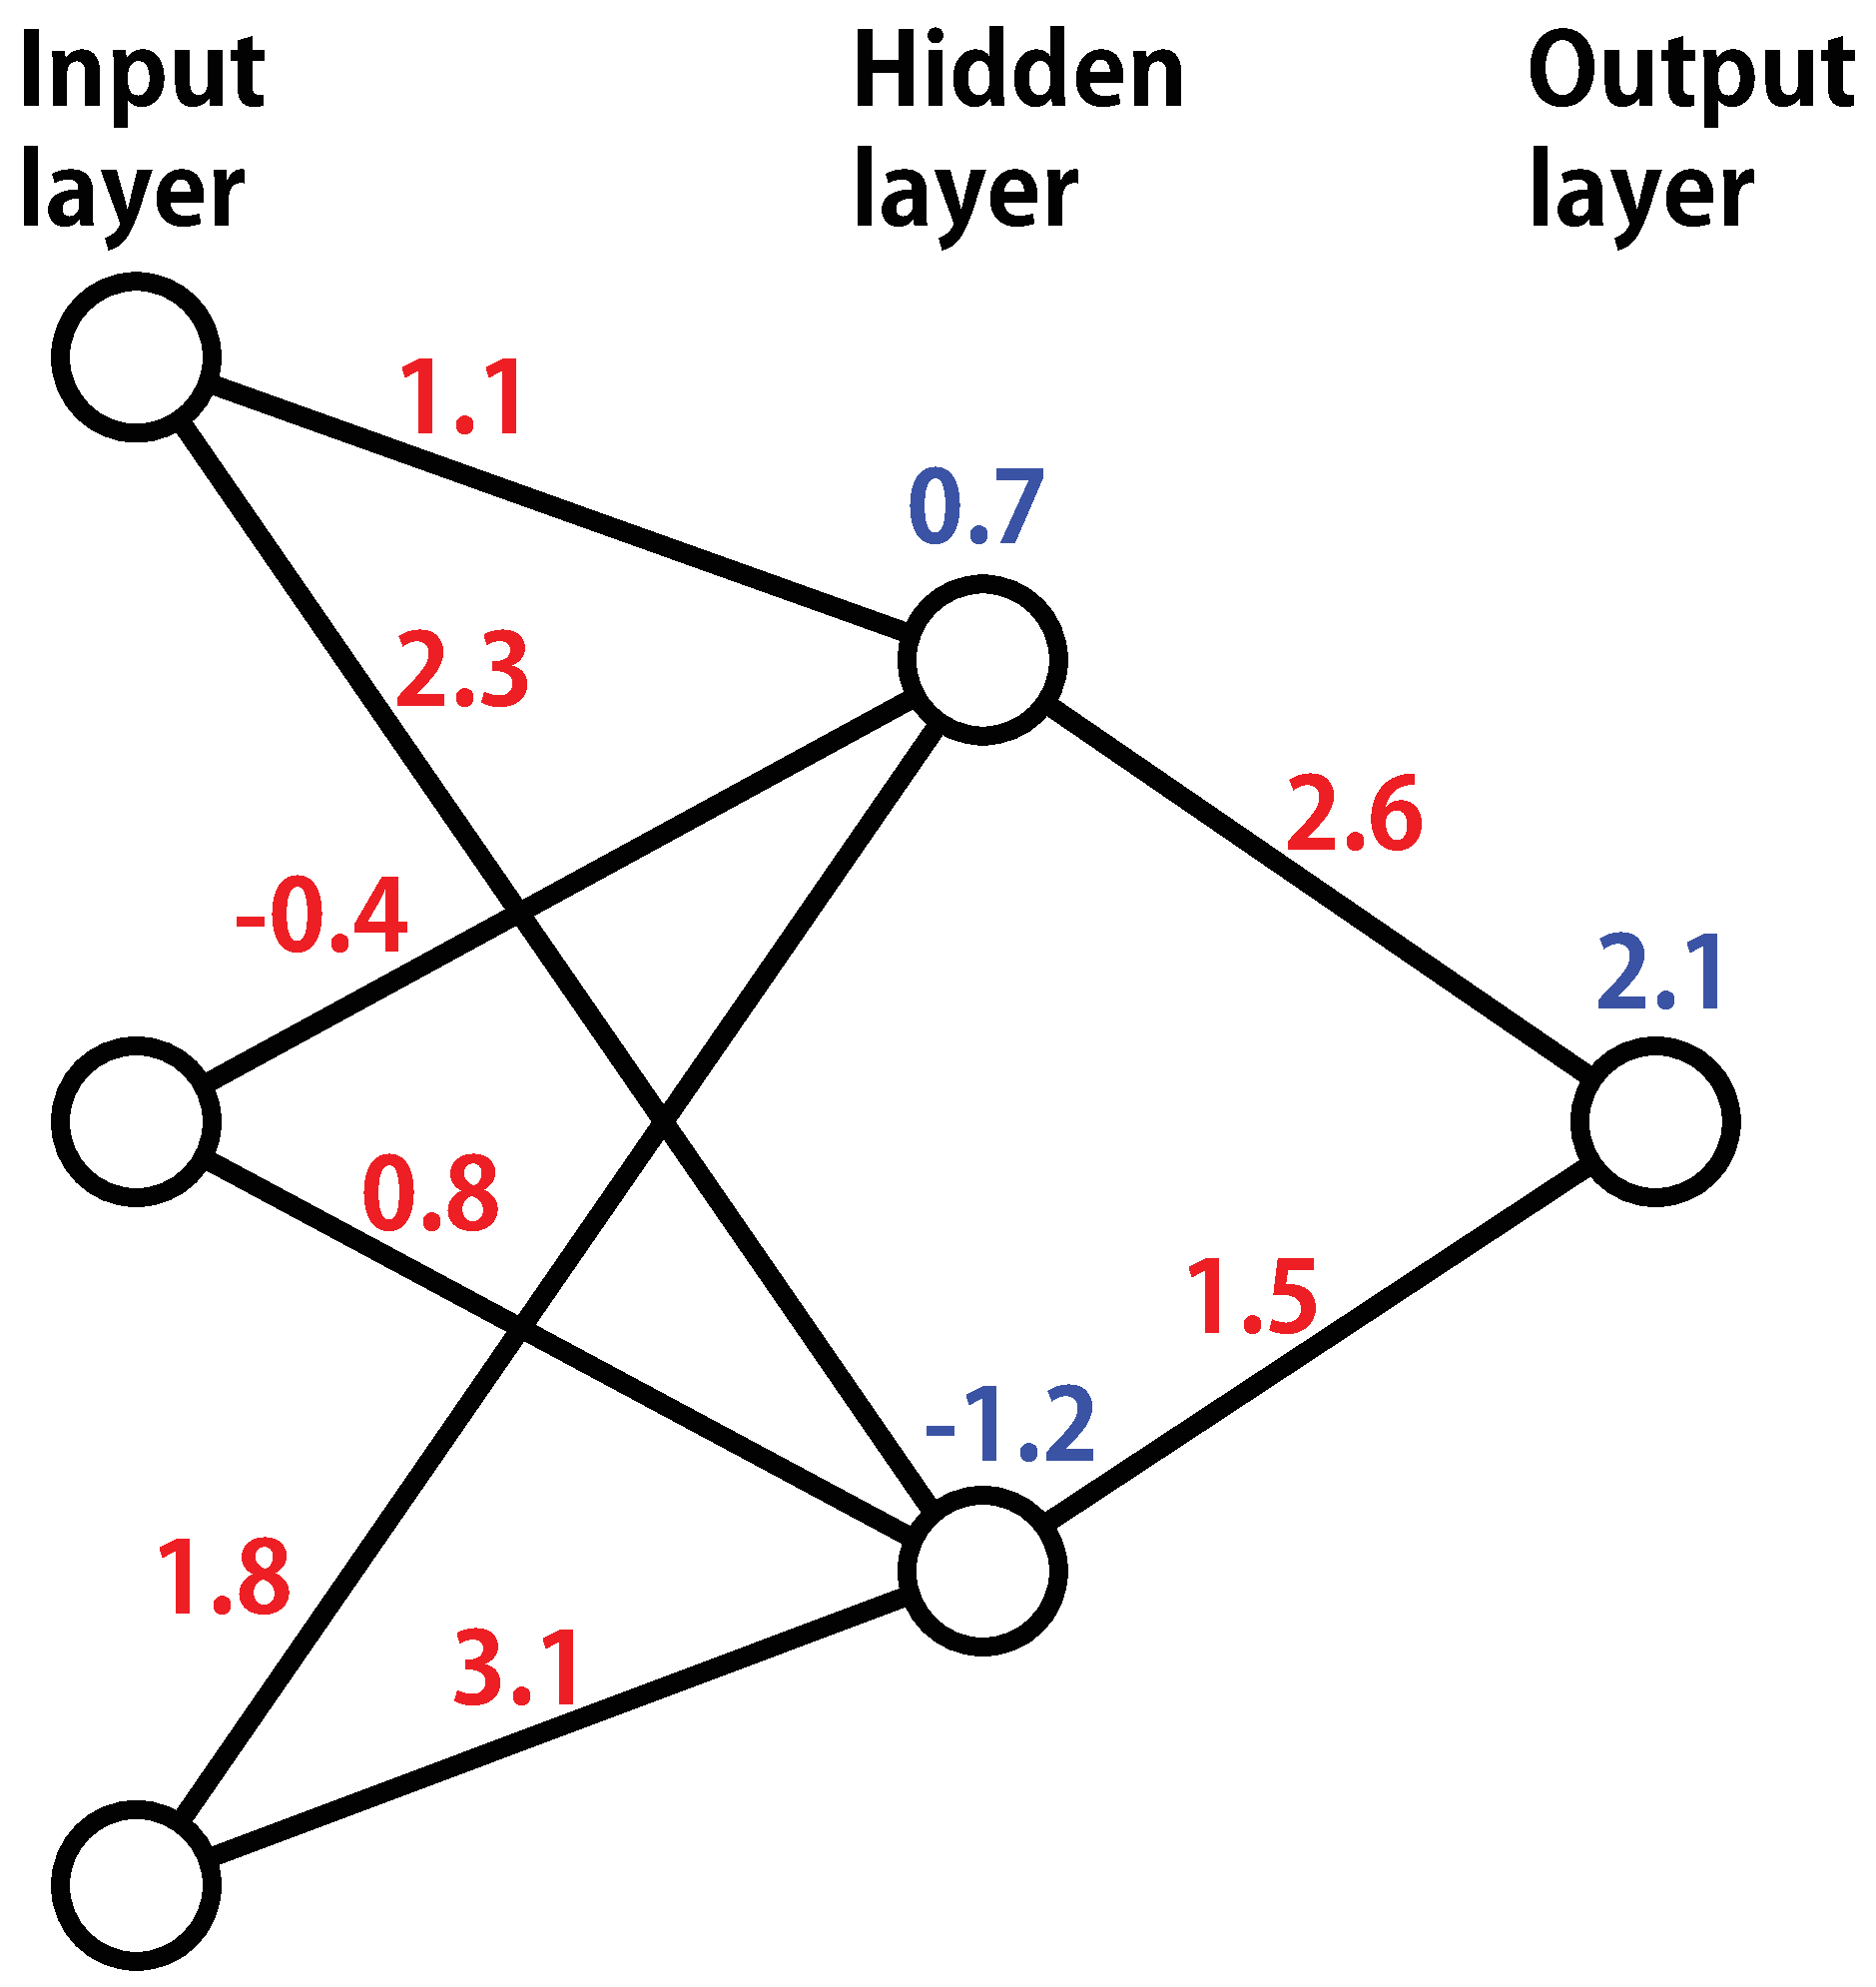
\includegraphics[width = 0.5 \textwidth]{./fig/ANN_sample_en}
  \caption{An example of an ANN.
    A red value indicates a weight, whereas
    a blue value indicates a bias.
    The direction of each arc is from left to right.}
  \label{fig:sample}
\end{figure}

\paragraph{Layers of an ANN.}
In the multi-layered perceptron model of ANNs,
an ANN consists of several \emph{layers}.
%
\begin{itemize}
  \item 
  The first layer is the {\em input layer}.
    Each node in the input layer is associated with a dimension of
    a feature vector (i.e., a descriptor). 
    Then the number of nodes in the input layer
    is equal to the number of dimensions of a feature vector. 
    
  \item 
  The subsequent layers (except the last one) are called
    {\em hidden layers}. A node in a hidden layer outputs a value
    based on the input values, where the input values
    are the outputs of all nodes in the previous layer.
    
  \item 
  The last layer is the {\em output layer} that has only one node.
    The output of this node is regarded as the output of the ANN. 
\end{itemize}

In the ANN of \figref{sample}, the input layer has three nodes.
This means that a feature vector should have three dimensions as well.
The ANN has one hidden layer that has two nodes.
The output layer has exactly one node. 

\paragraph{Weights.}
In ANNs, each edge is assigned a numerical value, called a {\em weight}.
The weights are determined by \emph{training} the ANN, 
based on the given data set. 

In \figref{sample}, the weights of edges are indicated in red. 


\paragraph{Biases.}
In ANNs, each node in the hidden layers and the output layer
is assigned a numerical value, which is called a {\em bias}.
The biases are determined together 
with the weights by training the ANN based on the given data set. 

In \figref{sample}, the biases of nodes are indicated in blue. 



\paragraph{Activation function.}
In ANNs, each node except the output one is assigned an activation function.
This function computes the output of the node
according to the weighted sum of the input values minus the bias of the node.

In this project, we use the Rectified Linear-Unit (ReLU) function
for the activation function of each node in the hidden layers.
This choice is due to Module 3, 
where it is assumed that the ReLU function is used
as an activation function for ANNs in Module 2.

\medskip

The process of deciding (appropriate) weights and biases
from a given data is called {\em learning}.

\invis{
\subsection{Files in the package}
\tabref{files} shows the list of files in the package of Module 2. 

\begin{table}[h!]
  \centering
  \caption{List of files in the package of Module 2}
  \label{tab:files}
  \begin{tabular}{lcll}
  \hline
  \bf File &\ \ & \multicolumn{2}{l}{\bf Description}\\
  \hline
  \verb|mol-infer_ANN.py| && \multicolumn{2}{l}{A Python script to train an ANN}\\
  &&\multicolumn{2}{l}{\bf (To proceed to Module 3,}\\
  &&\multicolumn{2}{l}{\bf it is necessary to run this script)}\\
  &&\multicolumn{2}{l}{$\bullet$ Used non-standard libraries: {\tt numpy, pandas, scikit-learn}}\\
  \hline
  \verb|predict_values.py| && \multicolumn{2}{l}{A supplementary Python script}\\
  &&\multicolumn{2}{l}{that predicts the value of a chemical property}\\
  &&\multicolumn{2}{l}{for molecules in a given data set}\\
  &&\multicolumn{2}{l}{(It is not necessary to run this script)}\\
  &&\multicolumn{2}{l}{$\bullet$ Used non-standard libraries: {\tt numpy, pandas}}\\
  \hline
  \multicolumn{4}{l}{\tt Manual\_Module\_2\_Cyclic\_jp.pdf}\\
  \multicolumn{4}{l}{\tt Manual\_Module\_2\_Cyclic\_jp.tex}\\
  %\multicolumn{4}{l}{\tt Manual\_Module\_2\_Cyclic\_improved\_jp.pdf}\\
  %\multicolumn{4}{l}{\tt Manual\_Module\_2\_Cyclic\_improved\_jp.tex}\\
  \multicolumn{4}{l}{\tt fig/ANN\_sample\_jp.eps}\\
  &&\multicolumn{2}{l}{PDF, \LaTeX\  source of the manual}\\
  &&\multicolumn{2}{l}{and the image file (Japanese version)}\\
  \hline
  \multicolumn{4}{l}{\tt Manual\_Module\_2\_Cyclic\_en.pdf}\\
  \multicolumn{4}{l}{\tt Manual\_Module\_2\_Cyclic\_en.tex}\\
  %\multicolumn{4}{l}{\tt Manual\_Module\_2\_Cyclic\_improved\_en.pdf}\\
  %\multicolumn{4}{l}{\tt Manual\_Module\_2\_Cyclic\_improved\_en.tex}\\
  \multicolumn{4}{l}{\tt fig/ANN\_sample\_en.eps}\\
  &&\multicolumn{2}{l}{PDF, \LaTeX\   source of the manual}\\
  &&\multicolumn{2}{l}{and the image file (English version)}\\
  \hline
  \multicolumn{4}{l}{\bf Data files for BP (boiling point)~\cite{pubchem}}\\
  \multicolumn{2}{l}{\tt data/BP.sdf} & \multicolumn{2}{l}{SDF file containing molecule data.}\\
  \multicolumn{2}{l}{\tt } & \multicolumn{2}{l}{This file is not explicitly treated in Module 2.}\\
  \multicolumn{2}{l}{\tt data/BP\_fv.csv} & \multicolumn{2}{l}{File containing feature vectors}\\
  \multicolumn{2}{l}{\tt } & \multicolumn{2}{l}{that are obtained by applying Module 1 to {\tt BP.sdf}}\\
  \multicolumn{2}{l}{\tt data/BP\_value.csv} & \multicolumn{2}{l}{File containing BP values of molecules}\\
  \multicolumn{2}{l}{\tt data/BP\_ANN.LOG} & \multicolumn{2}{l}{Log of executing {\tt mol-infer\_ANN.py}}\\
  \multicolumn{2}{l}{\tt } & \multicolumn{2}{l}{for the data set that consists of {\tt BP\_fv.csv, BP\_value.csv}}\\
  \multicolumn{4}{l}{\tt data/BP\_ANN\_biases.txt} \\
  \multicolumn{4}{l}{\tt data/BP\_ANN\_weights.txt} \\
  &&\multicolumn{2}{l}{The biases and weights of the constructed NN}\\
  \hline
  \end{tabular}
\end{table}

\newpage

\begin{table}[t!]
  \centering
  (Cont. of \tabref{files})
  
  \begin{tabular}{lcll}
  \hline
  \bf File &\ \ & \multicolumn{2}{l}{\bf Description}\\
  \hline
  \multicolumn{4}{l}{\bf Data files for HC (heat of combustion)~\cite{pubchem}}\\
  \multicolumn{2}{l}{\tt data/HC.sdf} & \multicolumn{2}{l}{(All are analogous to BP)}\\
  \multicolumn{2}{l}{\tt data/HC\_fv.csv} \\%& \multicolumn{2}{l}{Module 1 に{\tt HC.sdf}を入力して生成した特徴ベクトル}\\
  \multicolumn{2}{l}{\tt data/HC\_value.csv} \\%& \multicolumn{2}{l}{化合物のHC値を記したファイル}\\
  \multicolumn{2}{l}{\tt data/HC\_ANN.LOG} \\%& \multicolumn{2}{l}{{\tt HC\_fv.csv, HC\_value.csv}から成る訓練集合に対して}\\
  %&&\multicolumn{2}{l}{{\tt mol-infer\_ANN.py}を実行し, 学習したときのログ出力}\\
  \multicolumn{4}{l}{\tt data/HC\_ANN\_biases.txt} \\
  \multicolumn{4}{l}{\tt data/HC\_ANN\_weights.txt} \\
  %&&\multicolumn{2}{l}{学習されたNNにおける各ノードのバイアス, }\\
  %&&\multicolumn{2}{l}{および各枝の重み}\\
  \hline
  \multicolumn{4}{l}{\bf Data files for KOW (log Kow)~\cite{pubchem}}\\
  \multicolumn{2}{l}{\tt data/KOW.sdf} & \multicolumn{2}{l}{(All are analogous to BP)}\\
  \multicolumn{2}{l}{\tt data/KOW\_fv.csv} \\%& \multicolumn{2}{l}{Module 1 に{\tt KOW.sdf}を入力して生成した特徴ベクトル}\\
  \multicolumn{2}{l}{\tt data/KOW\_value.csv} \\%& \multicolumn{2}{l}{化合物のKOW値を記したファイル}\\
  \multicolumn{2}{l}{\tt data/KOW\_ANN.LOG} \\%& \multicolumn{2}{l}{{\tt KOW\_fv.csv, KOW\_value.csv}から成る訓練集合に対して}\\
  %&&\multicolumn{2}{l}{{\tt mol-infer\_ANN.py}を実行し, 学習したときのログ出力}\\
  \multicolumn{4}{l}{\tt data/KOW\_ANN\_biases.txt} \\
  \multicolumn{4}{l}{\tt data/KOW\_ANN\_weights.txt} \\
  %&&\multicolumn{2}{l}{学習されたNNにおける各ノードのバイアス, }\\
  %&&\multicolumn{2}{l}{および各枝の重み}\\
  \hline
  \multicolumn{4}{l}{\bf Data files for MP (melting point)~\cite{pubchem}}\\
  \multicolumn{2}{l}{\tt data/MP.sdf} & \multicolumn{2}{l}{(All are analogous to BP)}\\
  \multicolumn{2}{l}{\tt data/MP\_fv.csv} \\%& \multicolumn{2}{l}{Module 1 に{\tt MP.sdf}を入力して生成した特徴ベクトル}\\
  \multicolumn{2}{l}{\tt data/MP\_value.csv} \\%& \multicolumn{2}{l}{化合物のMP値を記したファイル}\\
  \multicolumn{2}{l}{\tt data/MP\_ANN.LOG} \\%& \multicolumn{2}{l}{{\tt MP\_fv.csv, MP\_value.csv}から成る訓練集合に対して}\\
  %&&\multicolumn{2}{l}{{\tt mol-infer\_ANN.py}を実行し, 学習したときのログ出力}\\
  \multicolumn{4}{l}{\tt data/MP\_ANN\_biases.txt} \\
  \multicolumn{4}{l}{\tt data/MP\_ANN\_weights.txt} \\
  %&&\multicolumn{2}{l}{学習されたNNにおける各ノードのバイアス, }\\
  %&&\multicolumn{2}{l}{および各枝の重み}\\
  \hline
  \end{tabular}

\end{table}
}

%%%%%%%%%%%%%%%%%%%%%%%%%%%%%%%%%%%%%%%%%%%%%%%%%%%%%%%%%%%%
%\clearpage
\section{A Quick Start}
\label{chap:quick2}

\paragraph{Training an ANN.}
The following command constructs an ANN from the dataset such that
\begin{itemize}
\item the set of feature vectors is written in \verb|instances/BP/BP_desc.csv|; and
\item the set of property values (BP in this case) is written in \verb|instances/BP/BP_values.txt|
\end{itemize}
\begin{oframed}
{\small
\noindent The symbol $\backslash$ at the end of the first line indicates that there
is no line break between the two lines, that is, they should be input without 
pressing the ``enter'' key.
\begin{verbatim}
$ python scikit_chemgraph_learning_lim.py ../instances/BP/BP_desc.csv\
 ../instances/BP/BP_values.txt output 20 10
\end{verbatim}
% \hfill $(\clubsuit)$
}
\end{oframed}

The constructed NN has two hidden layers,
where the numbers of nodes in these layers
are 20 and 10, respectively.
The weights of arcs are output to the file \verb|output_weights.txt|
and the biases of nodes are output to the file
\verb|output_biases.txt|.  
%
{\bf The files containing weights and biases are used in Module~3}. 


\paragraph{Predicting the property value of a given molecule.}
The property value of a molecule can be predicted by using a trained ANN.

The following command invokes a Python  script that
reads the information (edge weights and node biases)
of a trained ANN, and then uses each of the feature vectors
given in the file \verb|instances/BP/BP_desc.csv| as input to the
ANN's prediction function.
The edge weights of the trained ANN are read from the file \verb|output_weights.txt|,
and node biases are read from the file \verb|output_biases.txt|.
The output results 
are written to the file \verb|predicted.txt|. 

\begin{oframed}
  {\small
\noindent The symbol $\backslash$ at the end of the first line indicates that there
is no line break between the two lines, that is, they should be input without 
pressing the ``enter'' key.
\begin{verbatim}
$ python predict_values.py output_weights.txt output_biases.txt \
    instances/BP/BP_desc.csv predicted.txt
\end{verbatim}
}
  \end{oframed}

\begin{itemize}
\item Given an SDF file,
  one can generate the feature vectors of the molecules in the SDF
  by using the program in Module 1.
%\item 上のコマンドは, さらに上のコマンド$(\clubsuit)$で\verb|data/BP_fv.csv|を
%  特徴ベクトルとした訓練集合から学習したニューラルネットワークに関する \verb|output_weights.txt|および \verb|output_biases.txt|を用いるものとみなせば, 
%  訓練集合自身の化学的性質の値を推定していることになる. 
\item This script is supplementary, and it is not directly used in Modules~3 and~4. 
\end{itemize}


\section{Details in the Input and Output of the Program}
\label{chap:io2}

\subsection{Input}
\subsubsection{Feature vectors}
The feature vectors should be written in
a so-called {\bf FV format} to
a csv (comma-separated value) file. 
%
The feature vector generator in Module~1
generates a csv file in the FV format
from a given SDF.
As long as one uses the csv file generated in Module 1,
no problem should occur in Module 2. 

The explanation of the FV format was given in \chapref{io}.

\invis{
We explain the structure of the FV format using a simple example.  
\begin{oframed}
  {\small
\begin{verbatim}
CID,n,cs,ch,nsH
244,8,6,2,8
307,10,6,4,8
657014,11,7,1,18
16704,9,9,0,10
\end{verbatim}
}
\end{oframed}
\begin{itemize}
\item In the first line, the descriptor names should be written in comma-separated style.  
\item The first descriptor {\bf must be} CID (Compound ID).
  The CID values are not used to train an ANN, just for identification. 
\item In the above example,
  four descriptors are introduced: 
  \verb|n| (the number of atoms except hydrogens),
  \verb|cs| (core-size),
  \verb|ch| (core-height), and
  \verb|nsH| (the number of hydrogens). 
\item In each of the subsequent lines,
  the CID and the feature vector of one molecule
  should be specified in comma-separated style. 
\item The molecules {\bf need not be} ordered according to CID. 
\end{itemize}
}


\subsubsection{Property values}
The property values should be described in a csv file as follows.  
\begin{oframed}
  {\small
\begin{verbatim}
CID,a
307,11.2
244,-0.5
657014,98.124
16704,-12.8
117,5.3
\end{verbatim}
}
\end{oframed}
\begin{itemize}
\item {\bf The first line should be \verb|CID,a|. }
\item In each of the subsequent lines,
 the  CID and the property value of one molecule
  should be written in comma-separated style. 
\item The molecules need not be ordered with respect to CID. 
\end{itemize}
  
  
\subsection{Execution}

We use the Python script {\tt scikit\_chemgraph\_learning\_lim.py}
to train an ANN, as outlined in \chapref{quick}.


\subsubsection{Arguments}
We here revisit the commands 
explained in \chapref{quick2}.
\begin{oframed}
  {\small  
\begin{verbatim}
$ python scikit_chemgraph_learning_lim.py ../instances/BP/BP_desc.csv\
 ../instances/BP/BP_values.txt output 20 10
\end{verbatim}
%\verb|$ python mol-infer_ANN.py data/BP_fv.csv data/BP_value.csv output 20 10|
}
\end{oframed}
The meaning of each of the command-line parameters is as follows:
\begin{itemize}
\item Parameter~1: 
  A csv file that stores the feature vectors of chemical compounds,
  
\item Parameter~2: 
  A csv file that stores observed values of a chemical property/activity of chemical compounds,
  
\item Parameter~3: 
Filename where the weights and biases of a trained ANN will be stored,

\item Parameter~4: 
The number of nodes of hidden layers in the ANN, each layer separated by a space.
\end{itemize}

\invis{
If the Python script is invoked without supplying command-line arguments,
or in the case that there is a significant error in the arguments,
then a brief description of the command-line parameters will be printed.
\begin{oframed}
A verbatim output of the output of the program when invoked without any command-line parameters. The backslash symbol (\verb|\|) indicates that there is no actual line break. 
  {\small
\begin{verbatim}
$ python mol-infer_ANN.py 

usage: mol-infer_ANN.py (TrSet_FeatureVector.csv)(TrSet_TargetValue.csv) \
	    (Output_Name)(NN_Architecture)
                  
  - TrSet_FeatureVector.csv ... \
      The CSV file generated by our feature vector generator in Module 1.
  - TrSet_TargetValue.csv ... \
      The CSV file that contains target values.
    = The first column must contain CIDs.
    = The second column must contain target values and be named 'a'. 
    = All CIDs appearing in TrSet_FeatureVector.csv must be contained in \
	      TrSet_TargetValue.csv. 
  - OutputName_{biases,weights}.txt will be output. \
      They contain data on the constructed ANN. 
  - NN_Architecture ... Number of nodes in hidden layer(s).
\end{verbatim}
  }
  \end{oframed}
}

If the program is invoked with a proper set of command-line parameters,
then the training process of an ANN will begin.

To evaluate the performance of the trained ANN,
we use 5-fold cross-validation.
The ANN that achieved the highest coefficient of determination 
(${\rm R}^2$ score) for the test set over the five trials
is selected, and its weights and biases are stored
in a file.
Using the above example of parameter values,
where the value of parameter 3 is set to be \verb|output|,
the following two files will be written to disk:
\begin{itemize}
\item \verb|output_weights.txt| (stores the weights)
\item \verb|output_biases.txt| (stores the biases)
\end{itemize}
These two files are necessary in Module 3.


\paragraph{Caution on the data set}
The training set for training the ANN is given 
in the following two files
%
\begin{itemize}
\item a csv file with feature vectors of chemical compounds, and 
\item a csv file with observed values for a chemical property/activity.
\end{itemize}
Both files include the CID number of the corresponding chemical compound.
One important point to note is that
%
\begin{center}
  {\bf each of the CIDs in the former file must appear in the latter }
\end{center}
%
however, the opposite is not enforced.
In other words, there might be a chemical compound
for which an observed value of some property/activity
is listed in the latter file, but whose
feature vector is not included in the former.
Such values will be silently ignored.


\subsubsection{Hyper-parameters}

We use the Python  library {\tt scikit-learn}\footnote{\url{https://scikit-learn.org/stable/}}
and its {\tt MLPRegressor} tool
to do the training of an ANN as
a multi-layered perceptron.
After line 135 in the Python script 
\verb|scikit_chemgraph_learning_lim.py|, an instance of 
an \verb|MLPRegressor| is initialized, 
and its hyperparameters can be changed at this point.
Some of the various parameters are set as follows:
\begin{itemize}
\item \verb|activation|: \verb|`relu'|  \\
{\color{red}{\bf Attention:} 
If the trained neural network is to be used in Module 3 and afterward, 
the only possible choice here is
\verb|`relu'| (Rectified Linear Unit Function - ReLU).}
\item \verb|alpha|: $10^{-5}$
\item \verb|early_stopping|: \verb|False|
\item \verb|hidden_layer_sizes|: Passed as a command-line parameter at invocation
\item \verb|max_iter|: $10^{8}$
\item \verb|random_state|: 1
\item \verb|solver|: \verb|`adam'|
\end{itemize}


\subsection{Output}

We revisit the command issued as below, 
and explain the resulting output.
\begin{oframed}
  {\small
    \begin{verbatim}
$ python scikit_chemgraph_learning_lim.py ../instances/BP/BP_desc.csv\
 ../instances/BP/BP_values.txt output 20 10
\end{verbatim}
}
\end{oframed}

\subsubsection{Standard output}

When the above command is issued on the command prompt,
the results of the computation process will be displayed on the 
standard output.
An example of this output is stored in the file
\verb|instances/BP/BP_ANN.LOG|.

\invis{
%which is included together with
the program package and this note.
\begin{oframed}
  {\small
%\begin{verbatim}
% \end{verbatim}        
}
\end{oframed}

\begin{itemize}
\item  
First, the number of feature vectors, as well as the
number of descriptors are output.
Next comes the range 
(\verb|n range|, in the above example 5 -- 30)
of the number of non-hydrogen atoms (descriptor \verb|n|)
in the chemical
compounds in the training set, 
followed by the range 
(\verb|a range|,  31.5 -- 470.0 above)
of the observed 
chemical property/activity in the training data
(in this case, boiling point).

\item 
Following, the summary of each of the five runs of the
5-fold cross-validation is printed.

\item
Finally, the average of the calculation time,
R$^2$ score of the test set and MAE score of the test set over the 
five folds are printed.

\item 
In the above example, the ANN constructed 
in the third of the five folds had the 
highest R$^2$ score of 0.856697$\dots$, 
and therefore the values of its weights and
biases are written in the files
\verb|output_weights.txt| and \verb|output_biases.txt|, respectively.

\item
Note that a copy of each of the above files, 
\verb|output_weights.txt| and \verb|output_biases.txt|, 
is included in the set of files together with this note.
\end{itemize}
}

\subsubsection{Edge weights}
Following we explain the contents of the file
\verb|scikit_chemgraph_learning_lim.py|
that contains the values of the weights of the ANN.


For simplicity, let us assume that the ANN depicted
in \figref{sample} has been obtained after training.
The contents of the file with the weights of this ANN
would be as follows.
%
\begin{oframed}
{\small
\begin{verbatim}
3 2 1
1.1 2.3
-0.4 0.8
1.8 3.1
2.6
1.5
\end{verbatim}
}
\end{oframed}
%
\begin{itemize}
\item 
The first row gives the architecture of the ANN,
that is the number of nodes in each of its layers.
starting with the input layer, then the hidden layers, and
finally the output layer.

\item 
Starting from the second line and onward,
follow the weights of the ANN.
Each row gives the weights of the edges going out of a single node.
\end{itemize}


\subsubsection{Biases of nodes}
In a similar manner,
we give an explanation of the file that contains the
biases of the ANN obtained
by executing the Python script \verb|scikit_chemgraph_learning_lim.py|.

For sake of simplicity, again consider
the ANN depicted in \figref{sample}.
The values for the node biases of this ANN would be given as follows.
%
\begin{oframed}
{\small
\begin{verbatim}
0.7
-1.2
2.1
\end{verbatim}
}
\end{oframed}
Each row contains the bias value of a single node.
Note that the nodes of the input layer do not have biases.



\chapter{Module 3:
Inferring a 2-Lean Cyclic Chemical Graph with Bounded Branch-Height
from a Trained ANN Using MILP
}


\section{Outline}
\label{chap:Intro}

This chapter explains how to use an implementation of a mixed-integer
linear programming (MILP) formulation that can infer
a vector of graph descriptors given a target value and the 
weights and bias values of a trained artificial neural network (ANN).

The MILP is implemented in Python, 
using the PuLP modeling module of the 
COIN-OR package~\cite{PuLP1,PuLP2,PuLP3,PuLP4}.

\invis{
To begin with, we give a list of the files that accompany this note.

\begin{itemize}

\item Folder {\tt source\_code}\\
A folder containing four Python scripts that implement
an MILP formulation for inferring feature vectors
of cyclic chemical graphs from a trained ANN,
and files containing minimum and maximum values
of each descriptor
in the MILP formulation.

\begin{itemize}

\item {\tt ann\_inverter.py}\\
An implementation of an MILP formulation 
for the Inverse problem on  ANNs~\cite{AN19}.

\item {\tt cyclic\_graphs\_MILP\_ec\_id.py}\\
A Python script that contains functions to initialize the variables and prepare 
the constraints for an MILP
formulation for inferring cyclic chemical graphs with 
a prescribed topological structure~\cite{AN20}.

\item {\tt infer\_cyclic\_graphs\_ec\_id.py}\\
A Python script that prepares the data and executes 
the MILP formulation for given input data.
Further details on the use of this script
are given in Section~\ref{chap:Exp}.

\item {\tt read\_instance\_BH\_cyclic.py}\\
A Python script that contains necessary functions
to read the topological specification from a given textual file.

\item Folder {\tt topological\_description}\\
A folder containing six textual files each giving a chemical specification as detailed 
in~\cite{AN20}.
%
\begin{itemize}
 \item {\tt instance\_a.txt} 
 \item {\tt instance\_b1.txt} 
 \item {\tt instance\_b2.txt} 
 \item {\tt instance\_b3.txt}
 \item {\tt instance\_b4.txt}  
 \item {\tt instance\_c.txt} 
 \item {\tt instance\_d.txt} 
\end{itemize}

\item Folder {\tt ANN}\\
A folder containing information on trained artificial neural networks (ANNs) for three target properties:
Boiling point (Bp), Melting point (Mp), and Octanol/Water Partition Coefficient (Kow).
For each of the above three properties, ${\tt property} \in \{{\tt BP, MP, KOW}\}$ three files are provided:
%
\begin{itemize}
\item {\tt property\_desc.csv}\\
A comma-separated value file containing descriptors
used in the training of the ANN.

\item {\tt property\_biases.txt}\\
A file containing the values of the biases of a trained ANN.

\item {\tt property\_weights.txt}\\
A file containing the values of the weights of a trained ANN.
\end{itemize}
%
For each of the files, the data format is explained in Section~\ref{chap:InOut},
and an actual example is given in Section~\ref{chap:Exp}.

% \item {\tt fv4\_cyclic\_stdout.cpp}\\
% A C++ program that calculates the feature vector of 
% a chemical graph stored in SDF format.
% The input and output of this program are customized to work with 
% the Python script {\tt infer\_cyclic\_graphs\_ec\_id.py}
% in order to verify the descriptor values
% of the graph inferred as a solution to the MILP (if one exists).
% This source file should be compiled into an executable file
% with the name {\tt fv}.
% 
% \item {\tt fv}\\
% An executable binary file of the above C++ program.
% This executable has been compiled 
% by {\tt gcc} version 5.4.0
% on a PC running the Linux Mint 18.3 operating system.
%
\end{itemize}
\end{itemize}
}


The chapter is organized as follows.
Chapter~\ref{chap:Pre} gives an explanation 
of the used terms and notation.
%
Chapter~\ref{chap:InOut} explains the 
input and output data of the program,
and Chapter~\ref{chap:Exp} gives a concrete
example of input data and the results from a computation example.

% \newpage

\section{Terms and Notation}
\label{chap:Pre}
%
This section explains the terms and notation used in this note.


\begin{itemize}

\item {\bf Feature vector}\\
%
A {\em feature vector} stores numerical values of certain parameters,
called {\em descriptors}.
In this work, we choose graph-theoretical descriptors, such as number of 
non-hydrogen atoms, number of vertices of certain degree, etc.

\item {\bf Artificial neural network - ANN}\\
%
Artificial neural networks are one of the methods in machine learning.
They provide a means to construct a correlation function between 
pairs of feature vectors as input and target data as output.


\item {\bf Input, hidden, and output layer}\\
%
We deal with the multilayer perceptron model 
of feed-forward neural networks.
These neural networks are constructed of several {\em layers}.
First comes the \emph{input layer}, where each neuron takes as input
one value of the feature vector.
Next come the \emph{hidden layers}, where the 
values from the input layer are propagated in a feed-forward manner,
such that each node in one layer is connected to all the nodes of the next layer. 
Finally, the output is delivered at the \emph{output layer}.
We deal with predicting the value of a single target,
and hence we assume that the output layer comprises a single node.

\item {\bf Weights}\\
%
Each edge connecting two nodes in an ANN is assigned a real value,
called a \emph{weight}.
Part of the \emph{learning} process of ANNs is to determine values for each of the weights
based on known pairs of feature vectors and target values.

\item {\bf Biases}\\
Each node of an ANN except for the nodes in the input layer
is assigned a real value, called a {\em bias},
which, just like the edge weights, is determined through the learning process.


\item {\bf Activation function}\\
%
In an ANN, each node produces an output as a function, called the \emph{activation function}, 
of its input.
We assume that each node has the Rectified Linear-Unit (ReLU) function 
as its activation function,
which can be expressed exactly in the MILP formulation
for the inverse problem on ANNs~\cite{AN19}.
%https://scikit-learn.org/stable/modules/generated/sklearn.neural\_network.MLPRegressor.html

\item {\bf Mixed-Integer Linear Programming (MILP)}\\
%
A type of a mathematical programming problem
where all the constraints are given as linear expressions, and
some of the decision variables are required to take
only integer values.
For more details, see any standard reference, e. g.~\cite{LP}.


\item {\bf Graph} \\
An abstract combinatorial construction comprising
a finite set of {\em vertices}, and a finite set of {\em edges},
where each edge is a pair of vertices.
We treat {\em undirected} graphs,
i. e., graphs where edges are unordered pairs of vertices.
For more information, see e. g.~\cite{graph}.

\end{itemize}

% \newpage

\section{The Program's Input and Output}
\label{chap:InOut}

This section explains the format of the input and the output of the program.
Chapter~\ref{chap:section3_1} illustrates an example of the program's input format,
and Chapter~\ref{chap:section3_2} gives a concrete computational example.
Following, Chapter~\ref{chap:section3_3} illustrates an example of the program's output format,
and Chapter~\ref{chap:section3_4} gives a concrete computational example.


\subsection{Program Input}
\label{chap:section3_1}

This section gives an explanation of the input to the program.

First
the input requires three textual files containing \\
~~~~- the descriptor names, in csv format \\
~~~~- the weights and biases of a trained ANN in textual format.\\
For a common prefix {\tt TT} which the program accepts as a command-line parameter,
these files must be saved with file names {\tt TT\_desc.csv}, 
{\tt TT\_weights.txt}, and {\tt TT\_biases.txt}, for the files containing
the descriptor names, the weights, and the biases of a trained ANN, respectively.
%
Next, comes the target value for which we wish to infer 
a chemical graph based on the trained ANN given above.
Following is a chemical specification given in a textual file,
as described in~\cite{AN20}, 
as well as a filename prefix for the output files,  which are described in Chapter~\ref{chap:section3_4}.

Finally, comes a choice of MILP solver program to be used.
We can choose \\
~~~~- 1: CPLEX, a commercial MILP solver~\cite{cplex}, free for academic use. \\
(Note, in this case the parameter {\tt CPLEX\_PATH} in the file {\tt infer\_acyclic\_graphs.py}
must be set to the correct path of the CPLEX program executable file.) \\
~~~~- 2: CBC, a free and open-source MILP solver. 
It comes together with the PuLP package for Python~\cite{PuLP1}.




\subsection{Input Data Format}
\label{chap:section3_2}

This section presents an actual example of an input instance of the program.
In particular, we give a concrete example of the three input files
mentioned in Chapter~\ref{chap:section3_1}.

The purpose of this program is to calculate a feature vector that will produce a desired output from a 
given trained ANN.
Figure~\ref{fig:sample} gives an example of a trained ANN.

\invis{
\begin{figure}[H]
  \centering
  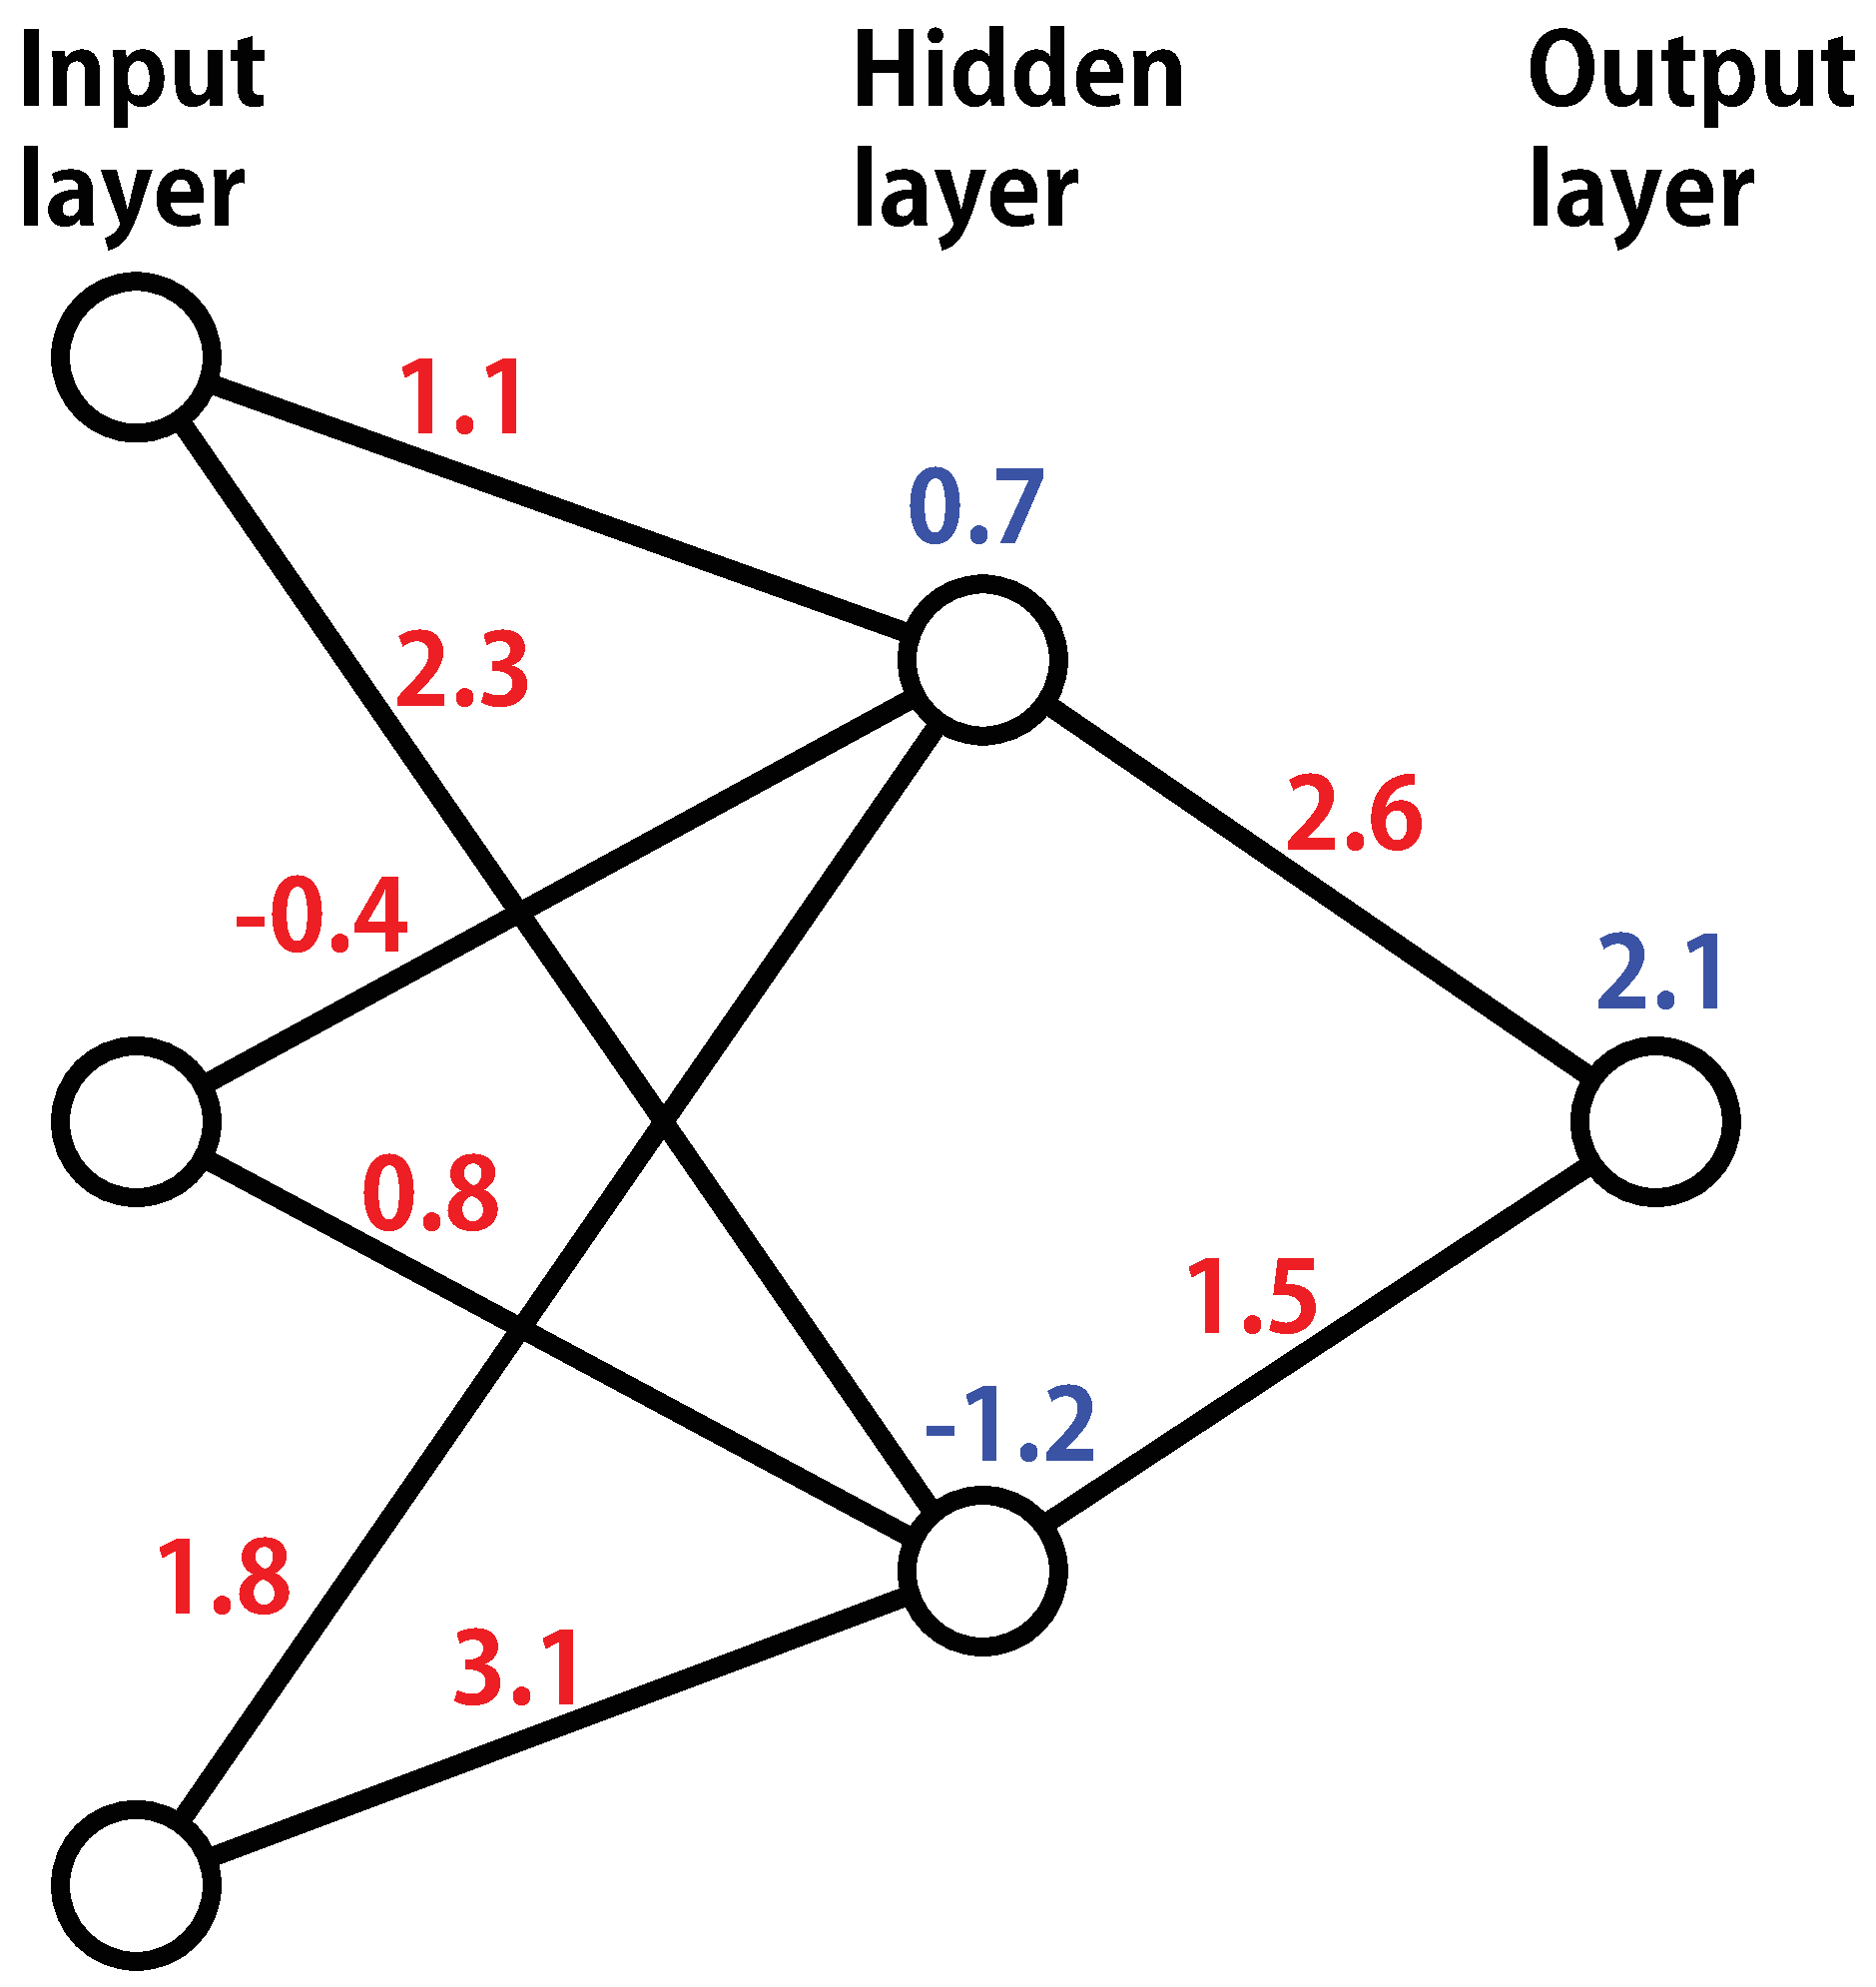
\includegraphics[width=0.5\textwidth]{./fig/ANN_sample_en}
  \caption{An example of a trained ANN.
		      The ANN's weights are given in red numbers, and
		      its biases in blue.
		    }
  \label{fig:sample}
\end{figure}
}

The information on the trained ANN is written in two text files, containing the information
on the ANN's weights and biases, respectively.
First, we give the structure of the file that contains the information on the ANN's weights.
The first line of this text file contains the information on the ANN's architecture, i. e., 
the number of nodes in each of its layers.
From the second row and onward
follows the information on the 
weights in the ANN.
Each row contains the weights of the edges that are incident to one node of the ANN,
first of the nodes in the input layer, and then for the nodes of the hidden layers.
Following is a textual example for the ANN given in Fig.~\ref{fig:sample}.

\bigskip

\begin{oframed}
{\bf Organization of the text file containing weight data}\\\\
%\bigskip\bigskip
3 2 1\\
1.1 2.3\\
-0.4 0.8\\
1.8 3.1\\
2.6\\
1.5\\
\end{oframed}

\bigskip


Next, comes the text file with the information on the ANN's biases.
The bias values from Fig.~\ref{fig:sample} are given below.

\bigskip

\begin{oframed}
{\bf Bias values}\\\\
%\bigskip\bigskip
0.7\\
-1.2\\
2.1\\
\end{oframed}

\bigskip

Last comes a text file containing data on the feature vector.
The first line of this file contains the names of the descriptors used in the feature vectors.
Following form the second row onward, are the numerical values of the descriptors for each chemical graph
in the training dataset, one row per chemical graph.
For an example, please check one of the files  {\tt TT\_desc.csv},  in the folder {\tt instances},
where ${\tt TT} \in \{{\tt BP, MP, KOW}\}$.



\subsection{Program Output}
\label{chap:section3_3}

This section gives an explanation of the output of the program.
If there exists an acyclic chemical graph with a feature vector that
would result with the given target value as a prediction of
the given trained ANN, the program will output the feature vector.
In case such a chemical graph does not exist, the program will report this.
The next section gives an explanation of the output of the program.


\subsection{Output Data Format}
\label{chap:section3_4}

This section describes the output data of the program as
obtained on a personal computer.

Once invoked, the program will print some messages to the standard error
stream, which appear on the terminal.
Once the MILP solver completes the computation,
the status of the computation is printed on the terminal.

\bigskip

\begin{oframed}
{\bf Text output on the terminal}\\\\
%\bigskip\bigskip
\begin{tabular}{l l}
 Initializing Time: 0.529                &         \# Written to {\tt stderr} \\
Start Solving Using CPLEX...      &       \# Written to {\tt stderr} \\
Status: Feasible 				&       \# Solution status \\
MILP y*: 223.856 				&      \# Calculated target value in the MILP  \\
ANN propagated y*: 223.856     &      \# Target value calculated by the trained ANN  \\
Solving Time: 52.534                     &      \# Time taken by the MILP solver \\
\end{tabular}



\end{oframed}

Finally, if there exists a feasible solution the program writes to disk two text files.
Recall that as a part of the input the program requires a filename
used for the output files. 
Assume that the supplied parameter is {\tt filename}.
Then, the resulting two text files are named \\
- {\tt filename.sdf} \\
- {\tt filename\_partition.sdf}. 

\noindent
The file {\tt filename.sdf} contains information
on the inferred chemical graph in the SDF (Structure Data File)
format.
For more information see the official documentation (in English) \\
\url{http://help.accelrysonline.com/ulm/onelab/1.0/content/ulm_pdfs/direct/reference/}\\
\phantom{\url{http://}} \url{ctfileformats2016.pdf} \\
for detail.

\noindent
The file {\tt filename\_partition.sdf} contains a 
decomposition of the cyclic graph from the 
file {\tt filename.sdf} into acyclic subgraphs,
as described in~\cite{AN20}.



\section{Invoking the Program and a Computational Example}
\label{chap:Exp}

This section explains how to invoke the program
and explains a concrete computational example.
Following is an example of invoking the
program {\tt infer\_cyclic\_graphs\_ec\_id.py}.

 


\subsection{Executing the Program}
\label{chap:Exp_1}

First make sure that the terminal is 
correctly directed to the location
%of the {\tt source\_code} folder, as described in Chapter~\ref{chap:Intro}. \\
of the {\tt bin} folder, as described in Chapter~\ref{chap:Intro}. \\

\noindent
{\tt 
 python  infer\_cyclic\_graphs\_ec\_id.py 
trained\_ann\_filename\_prefix
target\_value \\
 \phantom{python } 
 chemical\_specification
output\_file\_name
solver\_type
 }\\


As an example we use the target property Melting Point, 
that is, the files from the trained ANN with filename prefix {\tt MP},
target value 220,
the file {\tt instance\_1.txt} for a chemical specification,
and CPLEX~\cite{cplex} as an MILP solver (parameter value 1).

{\tt 
 python infer\_cyclic\_graphs\_ec\_id.py 
 ../instances/MP/MP
220 \\
 \phantom{python } 
 ../instances/chemical\_specification/instance\_a.txt
result
1
 }\\


By executing the above command, the following text should appear on the terminal prompt.

\bigskip

\begin{oframed}
{\bf Text output on the terminal}\\\\
%\bigskip\bigskip
 Initializing Time: 0.529  \\
Start Solving Using CPLEX...\\
Status: Feasible 		\\
MILP y*: 223.856 		\\
ANN propagated y*: 223.856 \\
Solving Time: 52.534       
\end{oframed}

The contents of the output files {\tt result.sdf} and
{\tt result\_partition.txt} are as follows.

\bigskip

\begin{oframed}
{\bf File {\tt result.sdf}}\\\\
\begin{verbatim}
 1
MILP_cyclic

 48 51  0  0  0  0  0  0  0  0999 V2000 
    0.0000    0.0000    0.0000 C   0  0  0  0  0  0  0  0  0  0  0  0
    0.0000    0.0000    0.0000 C   0  0  0  0  0  0  0  0  0  0  0  0
    0.0000    0.0000    0.0000 C   0  0  0  0  0  0  0  0  0  0  0  0
    0.0000    0.0000    0.0000 O   0  0  0  0  0  0  0  0  0  0  0  0
    0.0000    0.0000    0.0000 C   0  0  0  0  0  0  0  0  0  0  0  0
    0.0000    0.0000    0.0000 C   0  0  0  0  0  0  0  0  0  0  0  0
    0.0000    0.0000    0.0000 C   0  0  0  0  0  0  0  0  0  0  0  0
    0.0000    0.0000    0.0000 O   0  0  0  0  0  0  0  0  0  0  0  0
    0.0000    0.0000    0.0000 C   0  0  0  0  0  0  0  0  0  0  0  0
    0.0000    0.0000    0.0000 C   0  0  0  0  0  0  0  0  0  0  0  0
    0.0000    0.0000    0.0000 C   0  0  0  0  0  0  0  0  0  0  0  0
    0.0000    0.0000    0.0000 C   0  0  0  0  0  0  0  0  0  0  0  0
    0.0000    0.0000    0.0000 N   0  0  0  0  0  0  0  0  0  0  0  0
    0.0000    0.0000    0.0000 C   0  0  0  0  0  0  0  0  0  0  0  0
    0.0000    0.0000    0.0000 C   0  0  0  0  0  0  0  0  0  0  0  0
    0.0000    0.0000    0.0000 O   0  0  0  0  0  0  0  0  0  0  0  0
    0.0000    0.0000    0.0000 C   0  0  0  0  0  0  0  0  0  0  0  0
    0.0000    0.0000    0.0000 N   0  0  0  0  0  0  0  0  0  0  0  0
    0.0000    0.0000    0.0000 C   0  0  0  0  0  0  0  0  0  0  0  0
    0.0000    0.0000    0.0000 C   0  0  0  0  0  0  0  0  0  0  0  0
    0.0000    0.0000    0.0000 C   0  0  0  0  0  0  0  0  0  0  0  0
    0.0000    0.0000    0.0000 C   0  0  0  0  0  0  0  0  0  0  0  0
    0.0000    0.0000    0.0000 C   0  0  0  0  0  0  0  0  0  0  0  0
    0.0000    0.0000    0.0000 C   0  0  0  0  0  0  0  0  0  0  0  0
    0.0000    0.0000    0.0000 N   0  0  0  0  0  0  0  0  0  0  0  0
    0.0000    0.0000    0.0000 C   0  0  0  0  0  0  0  0  0  0  0  0
    0.0000    0.0000    0.0000 C   0  0  0  0  0  0  0  0  0  0  0  0
    0.0000    0.0000    0.0000 C   0  0  0  0  0  0  0  0  0  0  0  0
    0.0000    0.0000    0.0000 C   0  0  0  0  0  0  0  0  0  0  0  0
    0.0000    0.0000    0.0000 N   0  0  0  0  0  0  0  0  0  0  0  0
    0.0000    0.0000    0.0000 C   0  0  0  0  0  0  0  0  0  0  0  0
    0.0000    0.0000    0.0000 O   0  0  0  0  0  0  0  0  0  0  0  0
    0.0000    0.0000    0.0000 C   0  0  0  0  0  0  0  0  0  0  0  0
    0.0000    0.0000    0.0000 C   0  0  0  0  0  0  0  0  0  0  0  0
    0.0000    0.0000    0.0000 O   0  0  0  0  0  0  0  0  0  0  0  0
    0.0000    0.0000    0.0000 C   0  0  0  0  0  0  0  0  0  0  0  0
    0.0000    0.0000    0.0000 C   0  0  0  0  0  0  0  0  0  0  0  0
    0.0000    0.0000    0.0000 C   0  0  0  0  0  0  0  0  0  0  0  0
    0.0000    0.0000    0.0000 O   0  0  0  0  0  0  0  0  0  0  0  0
    0.0000    0.0000    0.0000 C   0  0  0  0  0  0  0  0  0  0  0  0
    0.0000    0.0000    0.0000 C   0  0  0  0  0  0  0  0  0  0  0  0
    0.0000    0.0000    0.0000 C   0  0  0  0  0  0  0  0  0  0  0  0
    0.0000    0.0000    0.0000 O   0  0  0  0  0  0  0  0  0  0  0  0
    0.0000    0.0000    0.0000 C   0  0  0  0  0  0  0  0  0  0  0  0
    0.0000    0.0000    0.0000 C   0  0  0  0  0  0  0  0  0  0  0  0
    0.0000    0.0000    0.0000 O   0  0  0  0  0  0  0  0  0  0  0  0
    0.0000    0.0000    0.0000 C   0  0  0  0  0  0  0  0  0  0  0  0
    0.0000    0.0000    0.0000 C   0  0  0  0  0  0  0  0  0  0  0  0
  1  2  1  0  0  0  0
  1 28  1  0  0  0  0
  1 29  1  0  0  0  0
  2  3  1  0  0  0  0
  2  4  2  0  0  0  0
  5  6  1  0  0  0  0
  5 28  1  0  0  0  0
  5 43  1  0  0  0  0
  6 29  2  0  0  0  0
  7  8  1  0  0  0  0
  7 27  1  0  0  0  0
  7 38  1  0  0  0  0
  8  9  1  0  0  0  0
  9 10  1  0  0  0  0
  9 31  1  0  0  0  0
 10 28  2  0  0  0  0
 11 21  1  0  0  0  0
 11 24  1  0  0  0  0
 12 13  1  0  0  0  0
 12 14  2  0  0  0  0
 12 18  1  0  0  0  0
 14 15  1  0  0  0  0
 15 16  2  0  0  0  0
 15 20  1  0  0  0  0
 17 18  1  0  0  0  0
 17 19  1  0  0  0  0
 19 20  1  0  0  0  0
 20 21  1  0  0  0  0
 21 23  1  0  0  0  0
 22 23  1  0  0  0  0
 22 25  1  0  0  0  0
 22 46  1  0  0  0  0
 23 24  2  0  0  0  0
 24 26  1  0  0  0  0
 25 27  1  0  0  0  0
 26 27  1  0  0  0  0
 29 30  1  0  0  0  0
 31 32  2  0  0  0  0
 31 33  1  0  0  0  0
 33 34  1  0  0  0  0
 33 35  1  0  0  0  0
 35 36  1  0  0  0  0
 36 37  3  0  0  0  0
 38 39  1  0  0  0  0
 39 40  1  0  0  0  0
 40 41  1  0  0  0  0
 40 42  1  0  0  0  0
 43 44  1  0  0  0  0
 44 45  3  0  0  0  0
 46 47  1  0  0  0  0
 47 48  3  0  0  0  0
M  END
$$$$
\end{verbatim}    
\end{oframed}

\bigskip

\begin{oframed}
{\bf File {\tt result\_partition.sdf}}\\\\
\begin{verbatim}
12
18
0 1
19
0 0
20
0 0
21
0 0
22
1 3
23
0 0
24
0 1
25
0 1
26
0 0
27
0 1
28
0 2
29
0 4
15
18 12 14 15 20
1 3
18 17 19
0 3
19 20
0 0
20 21
0 0
21 11 24
0 1
21 23
0 0
22 23
0 0
22 25
0 0
23 24
0 0
24 26
0 0
25 27
0 0
26 27
0 0
27 7 8 9 10 28
4 6
28 1 29
0 2
28 5 6 29
3 5
\end{verbatim}    
\end{oframed}



\chapter{Module 4:
Listing Chemical Isomers of a Given 2-Lean Cyclic Chemical Graph}

\section{Introduction}
\label{chap:intro}

This chapter explains how to use the program for listing
chemical isomers of a given 2-lean cyclic chemical graph~\cite{AN20}.

\invis{
The structure of files and folders of this module are 
as follows\\
\dirtree{%
.1 ./Module\_4.
.2 Manual\_Module\_4\_Cyclic\_en.pdf.
.2 Manual\_Module\_4\_Cyclic\_en.tex.
.2 Manual\_Module\_4\_Cyclic\_jp.pdf.
.2 Manual\_Module\_4\_Cyclic\_jp.tex.
.2 Pseudocode\_Graph\_Generation.pdf.
.2 files.
.3 Makefile.
.3 executables.
.4 linux.
.5 generate\_isomers.
.5 generate\_partition.
.4 osx.
.5 generate\_isomers.
.5 generate\_partition.
.4 windows.
.5 generate\_partition.exe.
.5 generate\_isomers.exe.
.3 instances.
.4 sample\_1\_partition.txt.
.4 sample\_1.png.
.4 sample\_1.sdf.
.3 main.
.4 readme.txt.
.4 generate\_partition.cpp.
.4 output.sdf.
.4 generate\_isomers.cpp.
.3 include.
.4 chemical\_graph.hpp.
.4 data\_structures.hpp.
.4 tools.hpp.
.4 cross\_timer.h.
.4 fringe\_tree.hpp.
}

\smallskip
The contents of each of the files is as follows.
%
\begin{itemize}		
 \item {\tt Manual\_Module\_4\_Cyclic\_en.pdf}\\
 This file.
 \item {\tt Manual\_Module\_4\_Cyclic\_en.tex}\\
 A \LaTeX~source file of this manual.
 \item {\tt Manual\_Module\_4\_Cyclic\_jp.pdf}\\
 The Japanese version of this manual.
 \item {\tt Manual\_Module\_4\_Cyclic\_jp.tex}\\
 A \LaTeX~source file of the Japanese version of the manual.
\item{ {\tt Pseudocode\_Graph\_Generation.pdf}}\\
  A pdf file with Pseudo-codes for the graph search algorithm.
 \item Folder {\tt files}
 \begin{itemize}
 \item {\tt Makefile} \\
	    Compilation directives for the C++ programs of this module.
    \item Folder {\tt executables}\\
    A folder that contains compiled executable files for 
    each of the architectures: linux, osx, and windows.
    
	\item Folder {\tt instances}\\
		A folder containing sample input instances.
		\begin{itemize}
			\item{\tt sample\_1.sdf}\\
			  A cyclic chemical graph with 20 vertices (non-Hydrogen atoms),
			    core size 18 and core height~1.
			\item{\tt sample\_1\_partition.txt}\\
			  A file containing partition information into acyclic subgraphs 
				of the cyclic chemical graph given in {\tt sample\_1.sdf}.
			\item{\tt sample\_2.sdf}\\
			  A cyclic chemical graph with 50 vertices, 
			    core size 24 and core height~6.
			\item{\tt sample\_2\_partition.txt}\\
			  A file containing partition information into acyclic subgraphs 
				of the cyclic chemical graph given in {\tt sample\_2.sdf}.
			\item{\tt sample\_3.sdf}\\
			  A cyclic chemical graph with 60 vertices, 
			    core size 31 and core height~4.
			\item{\tt sample\_3\_partition.txt}\\
			  A file containing partition information into acyclic subgraphs 
				of the cyclic chemical graph given in {\tt sample\_3.sdf}.
			\item{\tt sample\_4.sdf}\\
			  A cyclic chemical graph with 120 vertices, 
			    core size 60 and core height~4.
			\item{\tt sample\_4\_partition.txt}\\
			  A file containing partition information into acyclic subgraphs 
				of the cyclic chemical graph given in {\tt sample\_4.sdf}.
		\end{itemize}
    \item Folder {\tt main}\\
	    Folder containing source files written in the C++ programming language.
	    \begin{itemize}
		    \item{ \tt generate\_partition.cpp}\\
			    Functions for calculating a partition of a cyclic chemical graph into
			    acyclic subgraphs.
			    
		    \item{ \tt generate\_isomers.cpp}\\
			    Implements an algorithm for listing chemical isomers of
			    a 2-lean cyclic chemical graph.

	\item Folder {\tt include}\\
		A folder that contains related header files, written in C++.
		\begin{itemize}
			\item{chemical\_graph.hpp}\\
			  A header file that contains functions for manipulating 
			  chemical graphs.
			\item{cross\_timer.h}\\
				A header file that contains functions for measuring execution time.
				
			\item{data\_structures.hpp}\\
				Data structures implemented for storing chemical graphs.
				
			\item{debug.h}\\
				Used for debugging purposes.
				
			\item{fringe\_tree.hpp}\\
				Header file with functions for enumerating 2-fringe trees~\cite{AN20}.
				
			\item{tools.hpp}\\
				Various functions used in the implementation.
		\end{itemize}
		\end{itemize}
	  \end{itemize}
      \end{itemize}
}

%The remainder of this text is organized as follows.
The chapter is organized as follows.
Chapter~\ref{chap:term} explains some of the terminology used throughout the text.
Chapter~\ref{chap: partition} gives an explanation of the input and the output of
the program for calculating a partition of a cyclic chemical graph into
acyclic subgraphs, and provides a computational example.
Chapter~\ref{chap: main}
gives an explanation of the program for generating chemical isomers of
a given 2-lean cyclic chemical graph, explaining the input, output, and
presents a computational example.


% \newpage

\section{Terminology}
\label{chap:term}

This section gives an overview of the terminology used in the text.
%
\begin{itemize}
%
\item Chemical Graph\\
A graph-theoretical description of a chemical compound, 
where the graph's vertices correspond to atoms, and
its (multi) edges to chemical bonds.
Each vertex is colored with the chemical element of the atom it corresponds to,
and edges have multiplicity according to the corresponding bond order.
We deal with ``hydrogen-suppressed'' graphs, 
where none of the graph's vertices is colored as hydrogen.
This can be done without loss of generality,
since there is a unique way to saturate a hydrogen-suppressed chemical graph 
with hydrogen atoms subject to a fixed valence of each chemical element.


\item Feature vector\\
A numerical vector giving information such as the count of
each chemical element in a chemical graph.
For a complete information on the descriptors used in feature vectors for
this project, please see~\cite{AN20}.



\item Partition Information\\
Information necessary to specify the base vertices and edges, as well as the vertex and edge components
of a chemical graph.
For more details, please check~\cite{AN20}.
\end{itemize}


\section{Program for Calculating a Partition Into Acyclic Subgraphs}
\label{chap: partition}

\subsection{Input and Output}
\label{chap:InOut_p}

This section explains the input and output information of the 
program that is used to calculate a partition of a cyclic chemical graph
into acyclic subgraphs.
We call this program {\tt Partition}.
\invis{
  Following,
  Chapter~\ref{chap:Input_p} explains the input format, and
  Chapter~\ref{chap:Output_p} gives an explanation the output information of the program.
}

\subsubsection{The Program's Input}
\label{chap:Input_p}


The program {\tt Partition} takes two items as its input.

First, is a cyclic chemical graph, given as a ``structured data file,'' in  SDF format.
This is a standard format for representing chemical graphs.
For more details, please check the documentation at \\
\url{ http://help.accelrysonline.com/ulm/onelab/1.0/content/ulm_pdfs/direct/reference/} \\
\phantom{\url{ http://help.accelrysonline.com}}\url{/ctfileformats2016.pdf} 

Next,  is a filename of a text file where the information on 
a partition of the graph given in the SDF into acyclic subgraphs
calculated by the program will be saved.


\subsubsection{The Program's Output}
\label{chap:Output_p}

The output of this program is a 
partition into acyclic subgraphs of the cyclic chemical graph given in
the input.
The partition information is stored as a text file with filename as provided
in the input parameters.


\begin{oframed}
{\bf Output Format Example}\\\\
{\tt 4 \\
7 \# C \\
0 0 0 \\
15 \# C \\
0 0 0 \\
10 \# C \\
0 0 0 \\
16 \# C \\
0 0 0 \\
5 \\
7 4 3 5 6 9 2 15 \# C1C1N1C1C1C1O1C \\
0 1 0 \\
7 10 \# C2C \\
0 0 1 \\
10 12 14 13 11 7 \# C1C2C1C2C1C \\
0 0 1 \\
15 16 \# C2C \\
0 0 1 \\
16 18 20 19 17 15 \# C1C2C1C2C1C \\
0 0 1 \\}
\end{oframed}


Following, Table~\ref{tab:PartitionFormat}
gives a row-by-row explanation of the numerical information in the
above output file.


\bigskip
\begin{table}[H]
\begin{center} \caption{Structure of an Output File with Partition Information}
\label{tab:PartitionFormat}
  \begin{tabular}{l|l}
  Value in the file & Explanation \\ \hline \hline
{\tt  4} & Number of base vertices \\ \hline
{\tt  7 \# C} & The index of a base vertex in the input SDF and its element\\
{\tt  0 0 0} & Core height lower and upper bound; \\
{\tt  15 \# C} & \hspace{10mm} the vertex component can be created or not (0/1) \\
{\tt  0 0 0} & \\
{\tt  10 \# C} & \\
{\tt  0 0 0} & \\ 
{\tt  16 \# C} &\\ 
{\tt  0 0 0} & \\ \hline
{\tt  5} & Number of base edges \\ \hline
{\tt  7 4 3 5 6 9 2 15 \# C1C1N1C1C1C1O1C} & Indices of vertices in the base edge from the input SDF,\\
{\tt  0 1 0} & \hspace{10mm} their elements and bond multiplicities \\
{\tt  7 10 \# C2C} &\\ 
{\tt  0 0 1} &Core height lower and upper bound,\\
{\tt  10 12 14 13 11 7 \# C1C2C1C2C1C} &\hspace{10mm} the edge component can be created or not (0/1) \\
{\tt  0 0 1} & \\
{\tt  15 16 \# C2C} & \\
{\tt  0 0 1} & \\
{\tt  16 18 20 19 17 15 \# C1C2C1C2C1C} & \\
{\tt  0 0 1} & \\ \hline
  \end{tabular}
\end{center}
\end{table}



\subsection{Program Execution and Computation Example}
\label{chap:Example_p}

This section gives an explanation on how to compile and run the program,
as well as a concrete computational example of the program's execution.


\subsubsection{
Compiling and Executing the Program for Generating
a Decomposition of a Cyclic Graph  into Acyclic Graphs
}
\label{chap:compile_p}

A compiled executable that has been tested on\\
- linux \\
- osx \\
- windows (cygwin) \\
is included in the set of files.
In addition, we describe how the accompanying source files can be compiled.

\begin{itemize}
	\item {\em Computation environment}\\
		There should not be any problems when using an ISO C++11 compatible compiler. %
% 		The program has been tested on 
% 		Ubuntu Linux 20.04,  with the  g++ compiler version 9.3.
% 		If the compiler is not installed on the system, it can be installed with
% 		the following command.\\
% 		\verb|$ sudo apt install g++|
	\item {\em Compiling the program}\\
	      In the terminal, navigate to the {\tt files} subfolder.
	      Then, if the {\tt make} command is available on the system, the program can be simply compiled by typing \\
	      \verb|$ make generate_partition|\\
	      In case the {\tt make} command is not available, then the program can be compiled as \\	      
		\verb|$ g++ -o generate_partition ./main/generate_partition.cpp -O3 -std=c++11|\\
	\item {\em Executing the program}\\
		\verb|$ ./generate_partition instance.sdf instance_partition.txt|\\
		\verb|instance.sdf|  is an input SDF, 
		and a partition information as the output of the program is stored in the file
	  \verb|instance_partition.txt| .
\end{itemize}


\invis{
\subsubsection{Computational Example}
\label{chap:instance_p}

This section illustrates a concrete computational 
example of running the {\tt Partition} program.
We assume the following:
%
\begin{itemize}
\item Input file: {\tt sample\_1.sdf} from the folder {\tt instances} (see Sec.~\ref{chap:intro})
\item Output file to store the partition information: {\tt partition.txt}
\end{itemize}

Run the following command in the terminal to execute the program.

\bigskip

{\tt ./generate\_partition ./instances/sample\_1.sdf partition.txt}

\bigskip

After successfully executing the program, the contents of the file 
{\tt partition.txt} should be as follows.

\begin{oframed}
{\bf Contents of the file {\tt partition.txt}}\\\\
{\tt 4 \\
7 \# C \\
0 0 0 \\
15 \# C \\
0 0 0 \\
10 \# C \\
0 0 0 \\
16 \# C \\
0 0 0 \\
5 \\
7 4 3 5 6 9 2 15 \# C1C1N1C1C1C1O1C \\
0 1 0 \\
7 10 \# C2C \\
0 0 0 \\
10 12 14 13 11 7 \# C1C2C1C2C1C \\
0 0 0 \\
15 16 \# C2C \\
0 0 0 \\
16 18 20 19 17 15 \# C1C2C1C2C1C \\
0 0 0 \\}
\end{oframed}
}


\section{Program for Generating Chemical Isomers}
\label{chap: main}

\subsection{Input and Output of the Program}
\label{chap:InOut_m}

This section gives an explanation of the input and output
of the program that generates chemical isomers
of a given 2-lean chemical graph.
We call the program {\tt generate\_isomers}.
\invis{
Chapter~\ref{chap:Input_m} gives an explanation of the program's input, and
Chapter~\ref{chap:Output_m} of the program's output.
}

\subsubsection{The Program's Input}
\label{chap:Input_m}


The input to the {\tt generate\_isomers} program
consists of six necessary and one optional item. \\
First, comes information of a 2-lean chemical graph (in SDF format).\\
Second, comes a time limit in seconds on each of the stages of the program 
(for details, check the accompanying file with pseudo-codes of the algorithm).\\
Third is an upper bound on the number of {\em partial} feature vectors that the program stores
during its computation. \\
Fourth is the number of ``sample graphs'' that are stored per one feature vector.\\
Fifth is an upper limit on the number of generated output chemical graphs. \\
Sixth is a filename (SDF) where the output graphs will be written.\\
An optional parameter is a filename with a partition information of
the chemical graph given as the first parameter, and if given, it must be last
in the list of parameters.



\subsubsection{The Program's Output}
\label{chap:Output_m}

After executing the {\tt generate\_isomers} program,
the chemical isomers of the input graph will be written
in the specified SDF, and some information on the execution will be output on 
the terminal.
The information printed on the terminal includes:\\
 - a lower bound on the number of chemical isomers of the given input chemical graph, \\
 - the number of graphs that the program generated under the given parameters, and \\
 - the program's execution time.
 


\subsection{Executing the Program and a Computational Example}
\label{chap:Example_m}

This section gives a concrete computational example of the {\tt generate\_isomers} program.


\subsubsection{Compiling and Executing the {\tt generate\_isomers} Program}
\label{chap:compile_m}

Again, a compiled executable that has been tested on \\
- linux \\
- osx \\
- windows (cygwin) \\
is included in the set of files.
In addition, we describe how the accompanying source files can be compiled.

\begin{itemize}
	\item {\em Computation environment}\\
		There should not be any problems when using a ISO C++ compatible compiler. %
% 		The program has been tested on 
% 		Ubuntu Linux 20.04,  with the  g++ compiler version 9.3.
% 		If the compiler is not installed on the system, it can be installed with
% 		the following command.\\
% 		\verb|$ sudo apt install g++|
	\item {\em Compiling the program}\\
		If the {\tt make} command is available on the system, 
		then the program can be compiled in the {\tt files} folder by typing \\
		\verb|$ make generate_isomers|\\
		in the terminal.
		If the {\tt make} command is not available, then
		please run the following command in the terminal.\\
		\verb|$ g++ -o generate_isomers ./main/generate_isomers.cpp -O3 -std=c++11|\\
	\item {\em Executing the program}\\
		The program can be executed by running the following command in the terminal.\\
		\verb|$ ./generate_isomers instance.txt a b c d output.sdf instance_partition.txt|\\
		Above, {\tt generate\_isomers} is the name of the program's executable file, and the remaining command-line
		parameters are as follows: \\
		\verb|instance.txt|  a text file containing a chemical specification \\
		\verb|a| upper bound (in seconds) on the computation time, \\
		\verb|b| upper bound on the number of stored partial feature vectors, \\
		\verb|c| upper bound on the number of sample graphs stored per feature vector, \\
		\verb|d| upper bound on the number of output graphs, \\
		\verb|output.sdf| filename to store the output chemical graphs (SDF format), \\
		\verb|instance_partition.txt|  partition information of the input chemical graph.
\end{itemize}

\invis{
\subsubsection{Computational Example}
\label{chap:instance_p2}

We execute the {\tt generate\_isomers} program with the following parameters.

\begin{itemize}
\item Input graph: File {\tt sample\_1.sdf} from the folder {\tt instances} (see Sec.~\ref{chap:intro})
\item Time limit: 10 seconds
\item Upper limit on the number of partial feature vectors: 10000000
\item Number of sample graphs per feature vector: 5
\item Upper limit on the number of output graphs: 2
\item Filename to store the output graphs: {\tt output.sdf}
\item Partition information of the input graph: File {\tt sample\_1\_partition.txt} from the folder {\tt instances}.
\end{itemize}

Execute the program by typing the following command into the terminal (without a line break).

\bigskip


{\tt ./generate\_isomers ./instances/sample\_1.sdf 10 10000000 5 2} \\
\phantom{{\tt ./generate\_isomers ~~\,}} {\tt output.sdf ./instances/sample\_1\_partition.txt}	


\bigskip

Upon successful execution of the program, the following text should appear on the terminal.

\begin{oframed}
{\bf Output Written on the Terminal}\\\\
{\tt A lower bound on the number of graphs = 72\\
Number of generated graphs = 2\\
Total time : 0.00649s.}
\end{oframed}

\begin{oframed}
{\bf Contents of the file output.sdf}\\\\
{1 \\
BH-cyclic \\
BH-cyclic \\
 20 21  0  0  0  0  0  0  0  0999 V2000 \\
    0.0000    0.0000    0.0000  C  0  0  0  0  0  0  0  0  0  0  0  0 \\
    0.0000    0.0000    0.0000  C  0  0  0  0  0  0  0  0  0  0  0  0 \\
    0.0000    0.0000    0.0000  C  0  0  0  0  0  0  0  0  0  0  0  0 \\
    0.0000    0.0000    0.0000  C  0  0  0  0  0  0  0  0  0  0  0  0 \\
    0.0000    0.0000    0.0000  N  0  0  0  0  0  0  0  0  0  0  0  0 \\
    0.0000    0.0000    0.0000  C  0  0  0  0  0  0  0  0  0  0  0  0 \\
    0.0000    0.0000    0.0000  O  0  0  0  0  0  0  0  0  0  0  0  0 \\
    0.0000    0.0000    0.0000  C  0  0  0  0  0  0  0  0  0  0  0  0 \\
    0.0000    0.0000    0.0000  O  0  0  0  0  0  0  0  0  0  0  0  0 \\
    0.0000    0.0000    0.0000  C  0  0  0  0  0  0  0  0  0  0  0  0 \\
    0.0000    0.0000    0.0000  C  0  0  0  0  0  0  0  0  0  0  0  0 \\
    0.0000    0.0000    0.0000  C  0  0  0  0  0  0  0  0  0  0  0  0 \\
    0.0000    0.0000    0.0000  C  0  0  0  0  0  0  0  0  0  0  0  0 \\
    0.0000    0.0000    0.0000  C  0  0  0  0  0  0  0  0  0  0  0  0 \\
    0.0000    0.0000    0.0000  C  0  0  0  0  0  0  0  0  0  0  0  0 \\
    0.0000    0.0000    0.0000  C  0  0  0  0  0  0  0  0  0  0  0  0 \\
    0.0000    0.0000    0.0000  C  0  0  0  0  0  0  0  0  0  0  0  0 \\
    0.0000    0.0000    0.0000  C  0  0  0  0  0  0  0  0  0  0  0  0 \\
    0.0000    0.0000    0.0000  C  0  0  0  0  0  0  0  0  0  0  0  0 \\
    0.0000    0.0000    0.0000  C  0  0  0  0  0  0  0  0  0  0  0  0 \\
  1  3  2  0  0  0  0 \\
  1  5  1  0  0  0  0 \\
  1 16  1  0  0  0  0 \\
  2  4  2  0  0  0  0 \\
  2 11  1  0  0  0  0 \\
  2 20  1  0  0  0  0 \\
  3 13  1  0  0  0  0 \\
  4 17  1  0  0  0  0 \\
  5  6  1  0  0  0  0 \\
  6  7  1  0  0  0  0 \\
  7  8  1  0  0  0  0 \\
  8  9  1  0  0  0  0 \\
  8 10  1  0  0  0  0 \\
 10 11  1  0  0  0  0 \\
 11 12  1  0  0  0  0 \\
 13 14  2  0  0  0  0 \\
 14 15  1  0  0  0  0 \\
 15 16  2  0  0  0  0 \\
 17 18  2  0  0  0  0 \\
 18 19  1  0  0  0  0 \\
 19 20  2  0  0  0  0 \\
M  END \\
\$\$\$\$ \\
2 \\
BH-cyclic \\
BH-cyclic \\
 20 21  0  0  0  0  0  0  0  0999 V2000 \\
    0.0000    0.0000    0.0000  C  0  0  0  0  0  0  0  0  0  0  0  0 \\
    0.0000    0.0000    0.0000  C  0  0  0  0  0  0  0  0  0  0  0  0 \\
    0.0000    0.0000    0.0000  C  0  0  0  0  0  0  0  0  0  0  0  0 \\
    0.0000    0.0000    0.0000  C  0  0  0  0  0  0  0  0  0  0  0  0 \\
    0.0000    0.0000    0.0000  N  0  0  0  0  0  0  0  0  0  0  0  0 \\
    0.0000    0.0000    0.0000  C  0  0  0  0  0  0  0  0  0  0  0  0 \\
    0.0000    0.0000    0.0000  O  0  0  0  0  0  0  0  0  0  0  0  0 \\
    0.0000    0.0000    0.0000  C  0  0  0  0  0  0  0  0  0  0  0  0 \\
    0.0000    0.0000    0.0000  C  0  0  0  0  0  0  0  0  0  0  0  0 \\
    0.0000    0.0000    0.0000  C  0  0  0  0  0  0  0  0  0  0  0  0 \\
    0.0000    0.0000    0.0000  C  0  0  0  0  0  0  0  0  0  0  0  0 \\
    0.0000    0.0000    0.0000  O  0  0  0  0  0  0  0  0  0  0  0  0 \\
    0.0000    0.0000    0.0000  C  0  0  0  0  0  0  0  0  0  0  0  0 \\
    0.0000    0.0000    0.0000  C  0  0  0  0  0  0  0  0  0  0  0  0 \\
    0.0000    0.0000    0.0000  C  0  0  0  0  0  0  0  0  0  0  0  0 \\
    0.0000    0.0000    0.0000  C  0  0  0  0  0  0  0  0  0  0  0  0 \\
    0.0000    0.0000    0.0000  C  0  0  0  0  0  0  0  0  0  0  0  0 \\
    0.0000    0.0000    0.0000  C  0  0  0  0  0  0  0  0  0  0  0  0 \\
    0.0000    0.0000    0.0000  C  0  0  0  0  0  0  0  0  0  0  0  0 \\
    0.0000    0.0000    0.0000  C  0  0  0  0  0  0  0  0  0  0  0  0 \\
  1  3  2  0  0  0  0 \\
  1  5  1  0  0  0  0 \\
  1 16  1  0  0  0  0 \\
  2  4  2  0  0  0  0 \\
  2 11  1  0  0  0  0 \\
  2 20  1  0  0  0  0 \\
  3 13  1  0  0  0  0 \\
  4 17  1  0  0  0  0 \\
  5  6  1  0  0  0  0 \\
  6  7  1  0  0  0  0 \\
  7  8  1  0  0  0  0 \\
  8  9  1  0  0  0  0 \\
  8 10  1  0  0  0  0 \\
 10 11  1  0  0  0  0 \\
 11 12  1  0  0  0  0 \\
 13 14  2  0  0  0  0 \\
 14 15  1  0  0  0  0 \\
 15 16  2  0  0  0  0 \\
 17 18  2  0  0  0  0 \\
 18 19  1  0  0  0  0 \\
 19 20  2  0  0  0  0 \\
M  END \\
\$\$\$\$
}
\end{oframed}
}

% \addcontentsline{toc}{section}{\refname} 
\begin{thebibliography}{10}
	\bibitem{AN20}
	  T.~Akutsu and H.~Nagamochi.
	  A Novel Method for Inference of Chemical Compounds with Prescribed 
	  Topological Substructures Based on Integer Programming.
	  Arxiv preprint, arXiv:2010.09203
	
	  \bibitem{AN19} 
    T.~Akutsu and H.~Nagamochi.
    A Mixed Integer Linear Programming Formulation to Artificial Neural Networks,
    in Proceedings of the 2019 2nd International Conference on Information Science and Systems,
    pp.~215--220, https://doi.org/10.1145/3322645.3322683.
	  
	\bibitem{pubchem} HSDB in 
	PubChem \url{https://pubchem.ncbi.nlm.nih.gov} (accessed on February 1st, 2021)
    	  
    \bibitem{LP} J.~Matousek and B.~G\"{a}rtner.
				Understanding and Using Linear Programming. Springer, 2007.
				
    \bibitem{graph} M.~S.~Rahman.
				Basic Graph Theory. Springer, 2017.
    
    \bibitem{PuLP1} A Python Linear Programming API, \url{https://github.com/coin-or/pulp}.
    
    \bibitem{PuLP2} Optimization with PuLP, \url{http://coin-or.github.io/pulp/}.
    
    \bibitem{PuLP3} The Python Papers Monograph, \url{https://ojs.pythonpapers.org/index.php/tppm/article/view/111}.
    
    \bibitem{PuLP4} Optimization with PuLP, \url{https://pythonhosted.org/PuLP/}.
    
    \bibitem{cplex} IBM Cplex Optimizer \url|https://www.ibm.com/analytics/cplex-optimizer|.
	
\end{thebibliography}

\end{document}
